\documentclass{article}
\author{Giuliano Abruzzo}
\title{Distributed System Notes}
\usepackage{geometry}
\usepackage{float}
\usepackage{graphicx,array}
\usepackage{algorithmic,algorithm}
\usepackage{enumitem}
\usepackage[export]{adjustbox}
\usepackage{amsmath}
\usepackage{amssymb}
\newcolumntype{C}[1]{>{\let\newline\\\arraybackslash\hspace{0pt}}m{#1}}
\newcolumntype{L}[1]{>{\raggedright\let\newline\\\arraybackslash\hspace{0pt}}m{#1}}
\begin{document}

\maketitle
\newpage
\tableofcontents
\newpage
\section{Modelling Distributed System}
A \textbf{distributed system} is a set of \emph{entities, computers, machines} \textbf{communicating, coordinating} and \textbf{sharing resources} in order to reach a \textbf{common goal}, and appearing as a \textbf{single computing system}. To explain several situations in \emph{distributed systems}, we will use \textbf{distributed abstraction} cause they captures common \emph{properties} of a large range of \emph{systems}, and they prevent reinventing the same solution for variants of the same problem. We will use the Composition Model, where there are several elements represented as:\\
\begin{tabular}{C{4cm}  L{10.5cm}}
        \includegraphics[scale=0.6]{cattura.png} & \begin{itemize}
  \item \textbf{Request}: \emph{events} used by a \emph{component} to \textbf{request} a \emph{service} from another \emph{component};
  \item \textbf{Confirmation}: \emph{events} used by a \emph{component} to \textbf{confirm} the \emph{competition} of a \emph{request};
  \item \textbf{Indication}: \emph{events} used by a \emph{component} to \textbf{deliver information} to another \emph{component};
  \end{itemize}
\end{tabular}\\\\
We will use these three in \textbf{modules description} in the \emph{specification}. For a \emph{simple sync} and \emph{async Job Handler} we will have the following pseudocode:
\begin{figure}[H]
  \centering
  \includegraphics[scale=0.55, left]{cattura1.png}
\end{figure}
\begin{figure}[H]
  \centering
  \includegraphics[scale=0.55, left]{cattura2.png}
\end{figure}
\begin{figure}[H]
  \centering
  \includegraphics[scale=0.55, left]{cattura3.png}
\end{figure}
\hfill \break
If we need to show a \emph{Job transformation} and \emph{processing abstraction} we have to use another \emph{model}, with \textbf{two components}, a \textbf{Transformation Handler} and the \textbf{Job Handler}, in pseudocode: 
\begin{figure}[H]
  \centering
  \includegraphics[scale=0.48, left]{cattura4.png}
\end{figure}
\begin{figure}[H]
  \centering
  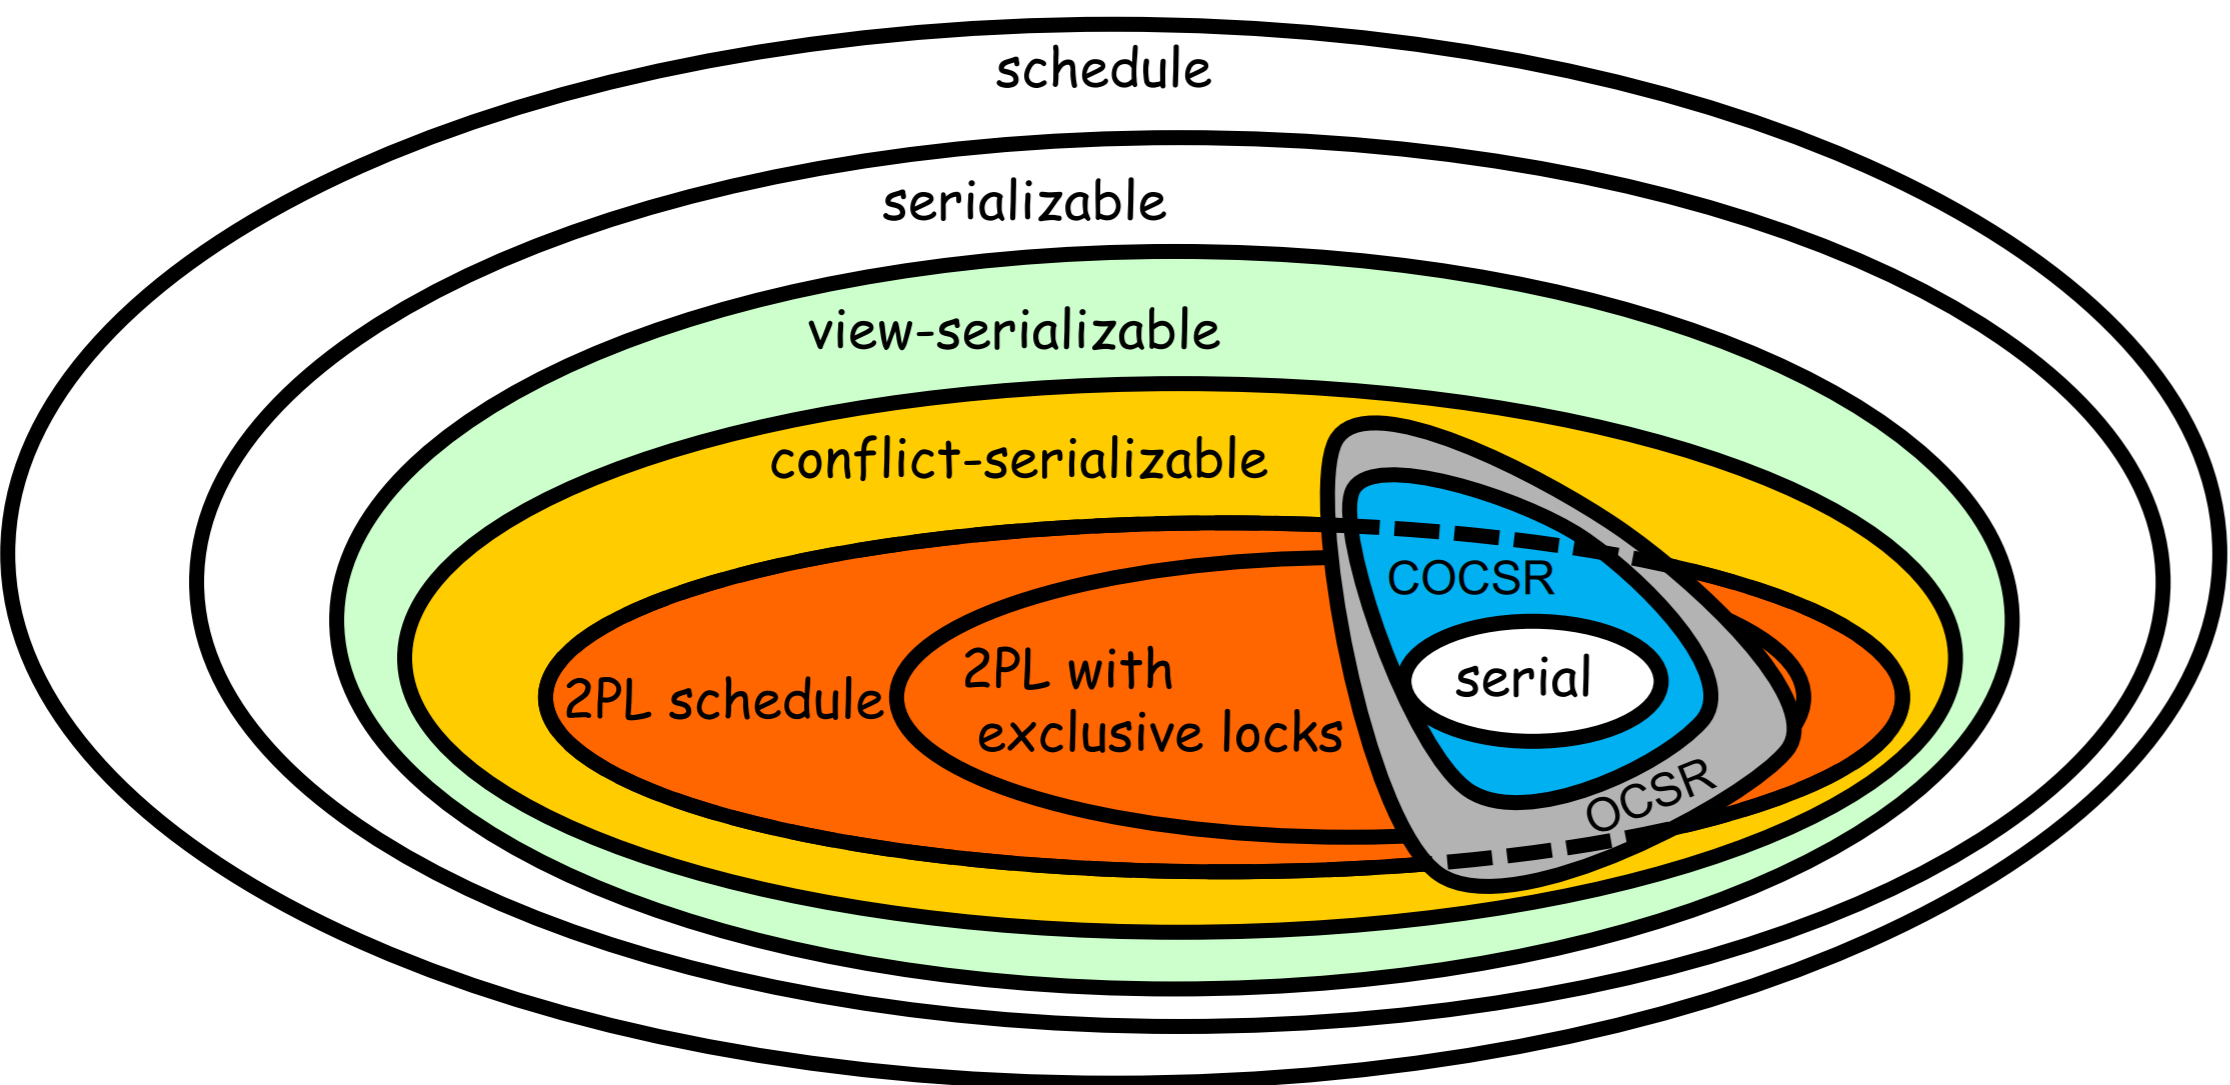
\includegraphics[scale=0.48, left]{cattura5.png}
\end{figure}
\hfill \break
Only the \emph{operations} referred to the \textbf{arrows entering} in the \textbf{Transformation Handler} are \emph{implemented}, because these are the \emph{operations} the \emph{Transformation Handler} has to handle. So, we write pseudocode which follows the given \emph{specification}, where \emph{operations} and \emph{properties} are listed. The \emph{bottom} and \emph{top} variables are used alongside with the \emph{buffer size} M to ensure that the limit of jobs that can be processed by the \emph{buffer} is not exceeded. Now we have two implements two exercises: 
\begin{figure}[H]
  \centering
  \includegraphics[scale=0.7, left]{cattura6.png}
\end{figure}
\begin{figure}[H]
  \centering
  \includegraphics[scale=0.62, left]{cattura7.png}
\end{figure}
\hfill\break
\textbf{Processes} in a \emph{Distributed System} often communicate through \textbf{messages}. We can represent a \textbf{distributed algorithm} as a series of \textbf{automata}, one per \emph{process}, which define how to react to a \emph{message}. The execution of a \emph{distributed algorithm} is represented by a sequence of steps executed by the \emph{processes}: 
\begin{figure}[H]
  \centering
  \includegraphics[scale=0.62]{cattura8.png}
\end{figure}
\emph{Distributed Algorithms} should have \textbf{two fundamental properties}:
\begin{itemize}
\item \textbf{Safety}: which states that the \emph{algorithm} should not behave in a wrong way;
\begin{itemize}
\item a \emph{safety property} is a property that can be violated at some time $t$ and never be satisfied again after that time;
\item a \emph{safety property} is a property such that, whenever it is violated in some execution $E$ of an \emph{algorithm}, there is a \emph{partial execution} ${E}'$ of $E$ such that the \emph{property} will be violated in any extension of $E$;
\end{itemize}
\item \textbf{Liveness}: which ensure that eventually something good happens;
\begin{itemize}
\item a \emph{liveness property} is a property of a \emph{distributed system} execution such that, for any time $t$, there is some hope that the property can be satisfied at some time ${t}' \geq t$.
\end{itemize}
\end{itemize}
There are three different \textbf{timing assumptions}:
\begin{itemize}
\item \textbf{Synchronous}: where there is a known \emph{upper bound} on the \emph{time} token for \emph{processing}, \emph{communication}, and a \emph{drift} of a \emph{local lock} with respect to \emph{real time};
\item \textbf{Asynchronous}: where there are no \emph{timing assumptions} on \emph{processes} and \emph{links}, but we can use \emph{logical clock} to measure \emph{time} with respect to \emph{communication}; 
\item  \textbf{Partially}: where there is an \emph{unknown time} $t$ after which the system behaves as a \emph{synchronous system}. It will be a period long enough to terminate the \emph{distributed algorithm};
\end{itemize}
\clearpage
\section{ Links}
\textbf{Links} are used to model the \emph{network component} of a \emph{distributed system}, in fact they connect pairs of \emph{processes}. We have three different types of \emph{link}:
\begin{itemize}
\item \textbf{Fair-loss links};
\item \textbf{Stubborn links};
\item \textbf{Perfect links};
\end{itemize}
The two \textbf{processes} linked can \emph{crash}, and the time taken to execute an \emph{operation} is \emph{bounded}, and the \textbf{messages} can be \emph{lost} and can take an indefinite time to reach the \emph{destination}. The \textbf{generic link interface} is:\\
\begin{tabular}{C{5cm}  L{9.5cm}}
   \includegraphics[scale=0.6]{cattura9.png} &  A \textbf{message} is typically received at a given port of the \emph{network} and stored in some \emph{buffer}, then some \emph{algorithm} is executed to satisfy the \emph{properties} of the \emph{link abstraction}, before the \emph{message} is actually \emph{delivered}. Remember, \textbf{Deliver} is different from \emph{receive}.
\end{tabular}\\\\
\subsection{Fair-Loss P2P link}
The \textbf{Fair-Loss point-to-point link} specification has two \emph{operations}, \emph{Send} and \emph{Deliver} and three \emph{properties}:
\begin{itemize}
\item \textbf{Fair-loss}: if a correct process \emph{p} infinitely often sends a message \emph{m} to a correct process \emph{q}, then \emph{q} delivers\emph{ m }an infinite number of times;
\item \textbf{Finite duplication}: if a correct processes \emph{p} sends a message \emph{m} a finite number of times to process \emph{q}, then \emph{m} cannot be delivered an infinite number of times by \emph{q};
\item \textbf{No creation}: if some process \emph{q} delivers a message \emph{m} with sender \emph{p}, then \emph{m} was previously sent to \emph{q} by \emph{p};
\end{itemize}
The \emph{sender} must take care of the \emph{retransmissions} if it wants to be sure that \emph{m} is delivered at its \emph{destination} and there is no guarantee that the \emph{sender} can stop the retransmissions of each \emph{message}, and each \emph{message} may be delivered more than once. 
\subsection{Stubborn P2P link}
The Stubborn point-to-point link has has two \emph{operations}, \emph{Send} and \emph{Deliver} and two \emph{properties}:
\begin{itemize}
\item \textbf{Stubborn delivery}: if a correct process \emph{p} sends a message \emph{m} once to a correct process, then \emph{q} delivers \emph{m} an infinite number of times; 
\item \textbf{No creation}: \emph{same as fair-loss p2p};
\end{itemize}
The implementation of the \textbf{Stubborn P2P link} is:
\begin{figure}[H]
  \centering
  \includegraphics[scale=0.5, left]{cattura10.png}
\end{figure}
\subsection{Perfect P2P link}
The \textbf{perfect link} solves all the issues presented above, in fact besides the \emph{No Duplication} and \emph{No Creation} it has another property:
\begin{itemize}
\item \textbf{Reliable delivery}: if a correct process \emph{p} sends a message \emph{m} to a correct process \emph{q}, then \emph{q} eventually delivers \emph{m};
\end{itemize}
\begin{figure}[H]
  \centering
  \includegraphics[scale=0.5, left]{cattura11.png}
\end{figure}
We can observe that the \emph{No duplication} is ensured by the last piece of pseudocode, thanks to the variable \emph{delivered}. \emph{No creation} is inherited, and \emph{Reliable delivery} derives from the whole schema, thanks to the \emph{perfect link} in particular which is built by chance to deliver \emph{messages} correctly. 
\clearpage
\section{Physical Time}
In a \emph{distributed system} \textbf{processes} run on different \emph{nodes} interconnected by mean of a \emph{network} and cooperate to complete a \emph{computation}. They communicate only through \emph{messages} and, as \emph{ordering} is require in such application, \textbf{time} is a \emph{critical factor} for \emph{distributed systems}. Each \emph{process} $p_i$ in a \emph{distributed} system runs on a single \emph{mono-processor machine} with no \emph{shared memory}, and they have a \emph{state} $s_i$, changed by the \emph{actions} during the \emph{algorithm execution}. Each \emph{process} generate a sequence of \emph{events}: 
\begin{itemize}
\item \textbf{Internal Event}: \emph{events} that transforms the \emph{process state};
\item \textbf{External Event}: \emph{send/receive};
\item $\mathbf{e_i^k}$: that represent the\emph{ k-th event} of the \emph{process} $p_i$;
\end{itemize}
We indicate with:
\begin{itemize}
\item $\rightarrow _i$ the \textbf{ordering relation} between two events $e$ and $e^{'}$;
\item $e \rightarrow _i e^{'}$ if and only if $e$ happened before $e^{'}$;
\end{itemize}
We call \textbf{local history} the sequence of \emph{events} produced by a \emph{process}, a \textbf{partial local history} a prefix of a local history, and \textbf{global history} the set containing every \emph{local history}. \emph{Events} can be \textbf{time-stamped} through \textbf{physical clocks} values, in fact in a \emph{single process} is always possible to order \emph{events}, but in a \emph{distributed system} in presence of \emph{network delay}, it is \textbf{impossible} to realize a \emph{common clock} shared among every \emph{process}. Anyway, it is possible to use \textbf{timestamps} in order to synchronize \emph{physical clocks} through \emph{algorithms} with a certain degree of approximation:
\[C_i(T)= \alpha\cdot H_i(t) + \beta \]\\
Where $C_i(t)$ represent the \textbf{software clock} and $H_i(t)$ represent the \textbf{hardware clock}, $\alpha$ and $\beta$ are two factors which approximate the result closer to guarantee \emph{monotonicity}. This \emph{software clock} is not generally completely \emph{accurate}, in fact it can be different from the \emph{real time} and at any \emph{process} due the precision of the approximation. We have to keep the \textbf{granularity}, also called \textbf{resolution}, the interval of time between two increments of the \emph{software clock}, of the \emph{software clock} smaller than the \emph{time difference} between two \emph{consequent events} so:
\[T_{resolution} < \Delta T_{\:between\: two\: notable\: events}\]
There are two parameters that effect \textbf{physical clocks}:
\begin{itemize}
\item \textbf{Skew}: the difference between two \emph{clocks}: $\left | C_i(t) - C_j(t) \right |$;
\item \textbf{Drift rate}: the \textbf{gradual misalignment} of once \emph{synchronized clocks} caused by the slight \emph{inaccuracies} of the time-keeping mechanism, for example the \emph{ordinary quartz clocks} deviate of 1 sec in 12 days;
\clearpage
\end{itemize}
\textbf{UTC} is the international standard for \emph{clock synchronization}, and we can have two types of \emph{synchronization}:
\begin{itemize}
\item \textbf{External Synchronization}:  
\begin{itemize}
\item In which \emph{processes} synchronize their \emph{clock} $C_i$ with an \emph{UTC source} $S$, in a way such that for each time interval: $\left | S(t) - C_i(t) \right | < D$ where $D$ is a \emph{synchronization bound};
\end{itemize}
\item \textbf{Internal Synchronization}:
\begin{itemize}
\item In which all the \emph{processes} synchronize their \emph{clock} $C_i$ between them with respect to $D$ in pairs so: $\left | C_i(t) - C_j(t) \right | < D$;
\end{itemize}
\end{itemize}
So, the \emph{clocks} that are \textbf{internally synchronized} are not necessarily \textbf{externally synchronized}, instead the \emph{clocks} that are \textbf{externally synchronized} are also \textbf{internally synchronized} with a \emph{bound} of $2\cdot D$. \\\\
An hardware clock is \textbf{correct} if its \emph{drift rate} is within a \emph{limited bound} of $p>0$:
\[1-p \leq \frac{dC}{dT} \leq 1+p\]
If we have a \textbf{correct hardware clock} H we can measure a \emph{time interval} $\left [ t, t^{'} \right ]$: 
\[(1-p)(t^{'}-t) \leq H(t^{'}) - H(t) \leq (1+p)(t^{'}-t)\]
\emph{Software clocks} have to be \textbf{monotone}: $t^{'} > t$, so $C(t^{'}) > C(t)$.
\subsection{Synchronization Algorithms}
\subsubsection{Christian's Algorithm}
\textbf{Christian's algorithm} is an \emph{external synchronization algorithm} which uses a \emph{time server} S that receives signal from an\emph{ UTS source}. It works also in an \emph{asynchronous system} in a probabilistically way. Is based on \textbf{message round trip} or \textbf{RTT}, and \emph{RTTs} must be small enough in order to obtain \emph{synchronization}. 
\begin{figure}[H]
  \centering
  \includegraphics[scale=0.5]{cattura12.png}
\end{figure}
\hfill \break
A process $p$ asks the current time through $m_r$ and receives $t$ in $m_t$ from S, and p will set its time to $t + \frac{RTT}{2}$, where $RTT$ is the round trip time experience by $p$. Is important to note that the \emph{time server} can crash or can be hacked. 
\clearpage 
\hfill \break
\textbf{Accuracy} of this \emph{algorithm} strongly depends of  $RTT$, and we can have two cases:\\
\begin{tabular}{C{11cm}  L{1cm}}
\begin{itemize}[leftmargin=*]
\item \textbf{Case 1}:
\begin{itemize}
\item In this case the \textbf{real reply time} is greater than \textbf{estimated time} that is $\frac{RTT}{2}$, so in particular is equal to $RTT - min$;
\item $\Delta = estimated - real = \frac{RTT}{2} - (RTT-min) = -(\frac{RTT}{2}-min)$;
\end{itemize}
\item \textbf{Case 2}:
\begin{itemize}
\item In this case the \textbf{real reply time} is smaller than \textbf{estimated time} that is $\frac{RTT}{2}$, so in particular is equal to $min$;
\item $\Delta = estimated - real = \frac{RTT}{2} - min = +(\frac{RTT}{2}-min)$;
\end{itemize} 
\end{itemize} &
\begin{figure}[H]
  \includegraphics[scale=0.5]{cattura13.png}
\end{figure}
\end{tabular}\\
So the the \textbf{accuracy} of \emph{Cristian's Algorithm} is $\pm (\frac{RTT}{2}-min)$ where $min$ is the \emph{minimum transmission delay}.
\subsubsection{Berkeley's Algorithm}
\textbf{Berkeley's Algorithm} is an \emph{internal synchronization algorithm} with a \textbf{master/slave structure} and is based on two \emph{steps}. In the first step gathering of all the \emph{clocks} from \emph{processes} and computation of the \emph{difference}, and in the second step there is the computation of the \emph{correction}. The accuracy of this protocol depends on the maximum round-trip time. If the \emph{master} crashes, another one is \emph{elected}, and it's tolerant to \emph{arbitrary behavior}, like a \emph{slave} that sends a wrong value, since the \emph{master} uses a \emph{threshold}. \\\\
The \textbf{master process} computes the differences $\Delta p_i$ between the\emph{ master clock} and the \emph{clock} of every process $p_i$ (even him self), after it compute the average, $avg$, of all the differences $\Delta p_i$ without considering \emph{faulty processes} (a process with a clock which differ from the \emph{master} one more than a \emph{threshold}) and at the end it computes the \textbf{correction} of each process (even \emph{faulty}) with the formula: $ADG_{p_i} = avg - \Delta p_i$. \\\\
When a \textbf{slaves process} receives the \emph{correction}, it is applied to the \emph{local clock}. If the \emph{correction} is negative, the \emph{process} doesn't adjust the value but it slow down its \emph{clock}, since decrementing can cause problems.
\subsubsection{Network Time Protocol}
The \textbf{NTP}, or \textbf{Network Time Protocol}, is a time service over \emph{Internet} that synchronizes \emph{clients} with \emph{UTC}. It's a standard for \emph{external clock synchronization} of \emph{distributed systems} and employs several \emph{security mechanisms} and is based on a \textbf{remote reading procedure} like the \emph{Cristian's Algorithm}. Furthermore it adds basic algorithm mechanisms for \emph{clustering}, \emph{filtering} and \emph{evaluating data quality}.
\clearpage
\hfill \break
\begin{tabular}{C{10.5cm}  L{6cm}}
It works with a \textbf{hierarchy}:
\begin{itemize}
\item \textbf{Primary server}: connected directly to \emph{UTC sources};
\item \textbf{Secondary server}: synchronized to \emph{primary servers};
\item \textbf{Synchronization subnet}: lowest \emph{level servers} in \emph{users computers};
\end{itemize}
This \textbf{hierarchy} in case of \emph{faults} is \emph{reconfigurable}. There are three modes of \textbf{synchronization}:
\begin{itemize}
\item \textbf{Multicast}: in which the \emph{server} periodically sends its \emph{actual time} to its \emph{leaves};
\item \textbf{Procedure Call}: in which the \emph{server} replies to request with its \emph{timestamp};
\item \textbf{Symmetrical}: in which we synchronize the pairs of \emph{time servers} using messages containing \emph{timing information};
\end{itemize}
& \includegraphics[scale=0.7]{cattura14.png}
\end{tabular}
It's important to note that \textbf{physical synchronization} doesn't work in \textbf{asynchronization system} as we completely make the \emph{bound logic} useless, in fact \emph{time for answer} is unpredictable.
\section{Logical Time}
\subsection{Logical clock}
As we said, \textbf{physical clock} are good if we have a precise estimation of \emph{delays}, but this can be hard, and often we want to know in which \emph{order} some \emph{events} happened and not the \emph{exact time} for each of them. Since in a \emph{distributed system} each \emph{system} has its own \emph{logical clock}, if \emph{clocks} are not aligned it's not possible to order \emph{events} generated by different \emph{processes}, so we need a reliable way to order \emph{events} and this is the \textbf{logical clock}. These \emph{clocks} are based on the \emph{causal relations} between events, and it's important to define two relations:
\begin{itemize}
\item $\rightarrow_i$ is the \textbf{ordering relation} between \emph{events} in a \emph{process} $p_i$;
\item $\rightarrow$ is the \textbf{happened-before} between any pairs of \emph{events};
\end{itemize}
We say that two \emph{events} $e$ and $e^{'}$ are in \textbf{happened-before} relation if:
\begin{itemize}
\item $\exists\; p_i\; |\; e \rightarrow_i e^{'}$;
\item $\forall$ message $m: send(m) \rightarrow receive(m)$;
\begin{itemize}
\item $send(m)$ is the event of \textbf{sending} a message $m$;
\item $receive(m)$ is the event of \textbf{receipt} of the same message $m$;
\end{itemize}
\item $\exists\; e, e^{'}, e^{''} \; | \; (e \rightarrow e^{''}) \wedge (e^{''} \rightarrow e^{'})$;
\end{itemize}
Where the last rule says that the \textbf{happened-before} relation is \textbf{transitive}. Using these rules we can define a \textbf{causal ordered sequence of events}, and if there are two \emph{events} that are not in \emph{happened-before} relation they are \textbf{concurrent} $(e \parallel e^{'})$. 
The \textbf{logical clock} is a \emph{software counting register} \textbf{monotonically} increasing its value and it's not related to the \emph{physical clock} in any way. We denote with $L_i(e)$ the \textbf{logical timestamp} assigned by the \emph{logical clock} by a \emph{process} $p_i$ to the \emph{event} $e$. There is a property that says: 
\[ if\; e \rightarrow e^{'}\; then\; L(e) < L(e^{'}) \]
There are two main implementations of the \textbf{logical clock}:
\subsubsection{Scalar Logical Clock}
Each \emph{process} $p_i$ initializes its \textbf{logical clock} $L_i = 0$, and $p_i$ increases its \emph{logical clock} of 1 when it generate an \emph{event} (send or receive): $L_i = L_i +1$ \\\\
\begin{tabular}{C{8cm}  L{6cm}}
When $p_i$ \textbf{sends} $m$:
\begin{itemize}
\item Create an event $send(m)$;
\item Increment $L_i$;
\item Timestamps $m$ with a $t=L_i$;
\end{itemize}
&
When $p_i$ \textbf{receives} $m$:
\begin{itemize}
\item Update $L_i = max(t, L_i)$;
\item Produce an event $receive(m)$;
\item Increment $L_i$;
\end{itemize}
\end{tabular}\\
As we said if  e $\rightarrow e^{'}$ then $L(e) < L(e^{'})$ but the contrary is not valid, so it possible that the two \emph{events} are \emph{concurrent}. So we cannot determine if two \emph{processes} are in \emph{happened-before} by analyzing \emph{scalar clocks} only. \\
\begin{tabular}{C{7.5cm}  L{7cm}}
\includegraphics[scale=0.8, left]{cattura15.png}
& In fact we can see that $L(e^3_1)<L(e^2_1)$ but: $e^2_1 \parallel e^3_1$;
\end{tabular}
\subsubsection{Vector Logical Clock}
Each \emph{process} has an \emph{array} of $N$ integers where $N$ is the number of \emph{processes} that are taken into consideration, this \emph{array} is called \textbf{Vector Clock}, and each \emph{process} maintains is own. \emph{Vector Clock} resolves the old problem cause here we have:
\[e \rightarrow e^{'}\; \mathbf{iff}\; L(e) < L(e^{'})\] 
Each process $p_i$ initialize its \textbf{vector clock} $V_i$: $V_i[j]=0\; \forall \; j= 1\;...\;N$, and $p_i$ increases $V_i[i]$ of 1 when it generates an event: $V_i[i] = V_i[i] +1$;
\\\\
\begin{tabular}{C{7cm}  L{8cm}}
When $p_i$ \textbf{sends} $m$:
\begin{itemize}
\item Create an event $send(m)$;
\item Increment $V_i$;
\item Timestamps $m$ with a $t=V_i$;
\end{itemize}
&
When $p_i$ \textbf{receives} $m$:
\begin{itemize}
\item Update $V_i[j] = max(t[j], V_i[j])\; \forall \; j=1\;...\;N$;
\item Produce an event $receive(m)$;
\item Increment $V_i$;
\end{itemize}
\end{tabular}\\ 
The implementation is like before, with the difference that the \emph{update} of the vector are done in an \emph{index} according to the \emph{event} that generated the \emph{message}. So $V_i[i]$ represents the numbers of \emph{events} produced by $p_i$, $V_i[j]$ represents the number of \emph{events} of $p_j$ that $p_i$ knows. Two \emph{events} are in \textbf{happened-before} only iff $V \leq V^{'} \wedge V \neq V^{'}$ so it must be $V < V^{'}$. \\
\begin{tabular}{C{7cm}  L{7cm}}
\includegraphics[scale=0.55, left]{cattura16.png}
&
\begin{align*}
\text{$\bullet$ event $e_1^1$}
\begin{bmatrix}
1\\0\\0
\end{bmatrix}
\text {$<$ event $e_2^1$}
\begin{bmatrix}
1\\1\\0
\end{bmatrix}
\text{so we have: $e_1^1\rightarrow e_2^1$}
\end{align*}
\begin{align*}
\text{$\bullet$ event $e_1^1$}
\begin{bmatrix}
1\\0\\0
\end{bmatrix}
\text {$\nless$ event $e_3^1$}
\begin{bmatrix}
0\\0\\1
\end{bmatrix}
\text{so we have: $e_1^1\parallel e_3^1$}
\end{align*}
\end{tabular}\\
Differently from \emph{Scalar Clock}, \textbf{Vector Clock} allows to determine if two \emph{events} are \emph{concurrent} or in \emph{happened-before}.
\subsection{Logical Time and Distributed Algorithms}
We have seen two mechanism to represent \textbf{logical time}, the \emph{scalar clock} and the \emph{vector clock}. We will now discuss how \textbf{logical-based algorithms} can be implemented in \emph{distributed systems}. But first the \textbf{mutual exclusion abstraction} specification are:
\begin{itemize}
\item \textbf{Mutual Exclusion}: at every time $t$ at most one \emph{process} $p$ is in \emph{critical section};
\item \textbf{No-Deadlock}: there always exists a \emph{process} $p$ able to enter in \emph{critical section};
\item \textbf{No-Starvation}: every \emph{process} $p$ requesting the \emph{critical section} eventually gets in;
\end{itemize}
\subsubsection{Lamport's algorithm}
In the \textbf{Lamport's algorithm} when a \emph{process} want to enter the \emph{critical section} sends a \emph{request message} to all the other, and a counter, \emph{timestamp}, is used for maintaining an history of the operations and this \emph{counter} is incremented for each \emph{event} and when a \emph{message} (even not related to \emph{mutual exclusion computation}) is \emph{sent} or \emph{received}. \\\\
Each \emph{process} $p_i$ uses a \textbf{data structure} composed of:
\begin{itemize}
\item $\mathbf{C_k}$: a \emph{counter} for process $p_i$;
\item $\mathbf{Q}$: a \emph{queue} maintained by $p_i$ where \emph{critical section requests} are stored;
\end{itemize}
The \textbf{algorithms rules} for \emph{process} $p_i$ are:
\begin{itemize}
\item \textbf{Access the CS}:  
\begin{itemize}
\item $p_i$ sends a \emph{request message} attaching $C_k$ to all \emph{processes} and adds its \emph{request} to $Q$;
\end{itemize}
\item \textbf{Request reception from $p_j$}:
\begin{itemize}
\item $p_i$ puts $p_j$ \emph{request} (\emph{timestamp} included) in its \emph{queue} and sends back an \emph{ACK} to $p_j$;
\end{itemize}
\item \textbf{$\mathbf{p_i}$ enters the CS iff}:
\begin{itemize}
\item $p_i$ has in its queue a \emph{request} with \emph{timestamp} $t$;
\item $t$ is the smallest \emph{timestamp} in the \emph{queue};
\item $p_i$ has already received an \emph{ACK} from another \emph{process} with $t^{'}>t$;
\end{itemize}
\item \textbf{Release of the CS}:
\begin{itemize}
\item $p_i$ sends a \emph{release message} to all the other \emph{processes} and deletes its own \emph{request} from the \emph{queue};
\end{itemize}
\item \textbf{Reception of a release message from $p_j$}:
\begin{itemize}
\item $p_j$ deletes $p_i$ \emph{request} from the \emph{queue};
\end{itemize}
\end{itemize}
\begin{figure}[H]
  \centering
  \includegraphics[scale=0.265]{cattura17.png}
\end{figure}
The \textbf{safety proof} can be explained as follow: let's suppose by \textbf{contradiction} that both the \emph{processes} $p_i$ and $p_j$ enter the \emph{critical section}, this means that both have received an \emph{ACK} from any other \emph{process} and the \emph{timestamp} has to be the smallest in the \emph{queue}:
\begin{itemize}
\item $t_i < t_j < ACK_i.ts$;
\item $t_j < t_i < ACK_j.ts$
\end{itemize}
So we have three cases:
\begin{itemize}
\item $p_j$ ACK arrives before $p_j$ request then $p_i$ can enter the CS without any problem;
\item $p_j$ ACK arrives after $p_j$ request but before $p_i$ ACK then $p_i$ enters the CS without any problem and sends its ACK after executing the CS;
\item Both processes receive the ACK when the two requests are in queue but \emph{mutual exclusion} is guaranteed by the \emph{total order} on the timestamps;
\end{itemize}
\textbf{Fairness} is satisfied because different \emph{requests} can be either in \emph{happened-before} or in \emph{concurrent} relation, so in the first case everything is done with the respect of that \emph{order}, while in the second case the \emph{CS access} can happened in any \emph{order}. In the worst case, this \emph{algorithm} needs $3(N-1)$ messages for the\emph{ CS execution}. 
\subsubsection{Ricart-Agrawala's algorithm}
Each \emph{process} has:
\begin{itemize}
\item \textbf{Replies} initially 0;
\item \textbf{State} $\in \left [ Requesting, CS, NCS \right ]$;
\item \textbf{Q} a \emph{queue} for \emph{pending requests} initially empty;
\item \textbf{Last\char`_Req};
\item \textbf{Num};
\end{itemize}
And the algorithm is:
\begin{figure}[H]
  \centering
  \includegraphics[scale=0.6]{cattura18.png}
\end{figure}
This algorithm sends the \emph{processes} into \textbf{critical section} based on the \emph{number} of the process, or on the basis of a \emph{deterministic function} that ensures the \textbf{total order}.
\clearpage
\section{Failure Detection \& Leader Election}
A system is \emph{synchronous}/\emph{asynchronous} or \emph{partially synchronous} depending on the \textbf{timing assumption}. If they are explicit we talk about a \emph{synchronous system}, otherwise it is \emph{asynchronous}. \emph{Partially systems} are the ones that need \emph{abstract timing} assumptions and we have two choices:
\begin{itemize}
\item Put assumption on the \emph{system model} (including \emph{links} and \emph{process});
\item Create a separate \emph{abstractions} that encapsulate \emph{timing assumptions};
\end{itemize}
\subsection{Failure Detector Abstraction}
A \textbf{failure detector abstraction} is a \emph{software module} used to detect \textbf{faulty processes}, it encapsulate \emph{timing assumptions} of a either \emph{partially synchronous} or\emph{ fully synchronous system}. It has two properties:
\begin{itemize}
\item \textbf{Accuracy}: that represents the ability to avoid \emph{mistakes};
\item \textbf{Completeness}: that represents the ability to detect all \emph{failures};
\end{itemize}
\subsubsection{Perfect Failure Detector}
\begin{figure}[H]
  \centering
  \includegraphics[scale=0.5, left]{cattura19.png}
\end{figure}
To prove the \textbf{correctness} we have to show that both the \emph{property} are satisfied. In this case they follow from the \emph{perfect point-to-point link}, in fact, if a \emph{process} crashes, it won't be able to send $HEARTBEATREPLY$ any more. If at the \emph{timeout} there is a \emph{process} that doesn't \emph{reply} to \emph{requests} it means that it has \emph{crashed}. 
\subsubsection{Eventually Perfect Failure Detector}
In the \textbf{Eventually perfect failure detector} there is an \emph{unknown time} $T$ after that \emph{crashes} can be \emph{accurately detected}. In the \emph{asynchronous period} (so the moments before $T$), the \emph{failure detector} can make mistake assuming \emph{correct processes} as \emph{crashed}, so the notion of \emph{detection} becomes \textbf{suspicious}.
\begin{figure}[H]
  \centering
  \includegraphics[scale=0.5, left]{cattura20.png}
\end{figure}
\hfill \break
As we see from the \textbf{specification}, a $<>P$ can mistakenly \emph{suspect} a \emph{process} but is able to \emph{restore} it as soon as possible, as it receives a \emph{reply}, also updating the \emph{timeout}. This can happen when the chosen \emph{timeout} is too short. If a \emph{process} $q$ \emph{crashes} and stops to send \emph{replies}, $p$ doesn't change its \emph{judgment} anymore. 
\clearpage
\subsection{Leader Election}
\subsubsection{Perfect Leader Election}
Sometimes, we may be more interested in knowing if a \emph{process} is \textbf{alive} instead of monitoring \emph{failures}. We can use a different oracle which reports a \emph{process} that is alive called \textbf{Leader Election} module. In the \textbf{perfect leader election} we use the \emph{perfect failure detector}:
\begin{figure}[H]
  \centering
  \includegraphics[scale=0.5, left]{cattura21.png}
\end{figure}
\subsubsection{Eventual Leader Election}
If the \emph{failure detector} is not perfect we talk about \textbf{eventual leader election}:
\begin{figure}[H]
  \centering
  \includegraphics[scale=0.6, left]{cattura22.png}
\end{figure}
\begin{figure}[H]
  \centering
  \includegraphics[scale=0.7, left]{cattura23.png}
\end{figure}
This ensures that, eventually, \emph{correct processes} will elect the same \emph{correct process} as their \textbf{leader}. It doesn't guarantee that \emph{leaders} may change in an arbitrary period of time, and that many \emph{leaders} might be elected during the same period of time without having \emph{crashed}. Once a \emph{unique leader} is determined and doesn't change again, we say that the leaser has \textbf{stabilized}. 
\subsubsection{Leader Election with Fair Lossy Links}
If we have a\textbf{ fair-loss link} we need to convert the whole schema and we need to use \textbf{crash-recovery} and \textbf{timeouts}:
\begin{figure}[H]
  \centering
  \includegraphics[scale=0.8, left]{cattura25.png}
\end{figure}
The last piece of code, in the \emph{fill deliver} \emph{event}, we will replace the number of \textbf{epoch} of a \emph{process} that crashed again.
\begin{figure}[H]
  \centering
  \includegraphics[scale=0.8, left]{cattura24.png}
\end{figure}
\textbf{Exercise 1}
\begin{figure}[H]
  \centering
  \includegraphics[scale=0.75, left]{cattura26.png}
\end{figure}
\begin{algorithm}[H]
\renewcommand{\thealgorithm}{}
\floatname{algorithm}{}
\caption{\textbf{Exercise 1.1}}
The answer is \textbf{yes}, because we can implement it on the \emph{process} that has all the \emph{links} of \textbf{channel A}. So, in that case when the \emph{timeout} will end if a \emph{process} didn't send a \emph{reply} we know for sure that it has \textbf{crashed}. \\
\begin{algorithmic}  
\STATE \textbf{Init:}
\STATE correct$_i$ = \{$p_1,p_2,p_3,p_4$\}
\STATE alive$_i$ = $\varnothing$
\STATE detected$_i$ = $\varnothing$
\STATE \textbf{for each} $p_j \in$ correct$_i$ \textbf{do}:
\STATE \hskip4.0em \textbf{trigger} $send(HearthBeatRequest, i)$ to $p_j$
\STATE $start(timer_1)$ \newline
\STATE \textbf{upon event}  $deliver(HearthBeatRequest, j)$ from $p_j$
\STATE \hskip4.0em \textbf{trigger} $send(HearthBeatReply, i)$ to $p_j$\newline
\STATE \textbf{upon event}  $deliver(HearthBeatReply, j)$ from $p_j$
\STATE \hskip4.0em alive$_i$ = alive$_i \cup \{p_j\}$\newline
\STATE \textbf{when}  $timer_1 = 0$
\STATE \hskip4.0em \textbf{for each} $p_j \in correct_i$ \textbf{do}:
\STATE \hskip8.0em \textbf{trigger} $send(ALIVE_LIST,alive_i, i)$ to $p_j$
\STATE \hskip4.0em $start(timer_2)$\newline
\STATE \textbf{when}  $timer_2 = 0$
\STATE \hskip4.0em \textbf{for each} $p_j \in correct_i$ \textbf{do}:
\STATE \hskip8.0em \textbf{if} $p_j \notin$ alive$_i \wedge p_j \notin$ detected$_i$
\STATE \hskip12.0em detected$_i$ = detected$_i \cup \{ p_j \}$
\STATE \hskip12.0em \textbf{trigger} $crash(p_j)$
\STATE \hskip4.0em alive$_i$ = $\varnothing$
\STATE  \hskip4.0em \textbf{for each} $p_j \in$ correct$_i$ \textbf{do}:
\STATE \hskip8.0em \textbf{trigger} $send(HearthBeatRequest, i)$ to $p_j$
\STATE \hskip4.0em $start(timer_1)$\newline
\end{algorithmic}
\end{algorithm}

\begin{algorithm}[H]
\renewcommand{\thealgorithm}{}
\floatname{algorithm}{}
\caption{\textbf{Exercise 1.2}}
We can't cause once the \emph{process} that has all the \textbf{channels A }\emph{fails}, it's not \emph{guaranteed} that all the \emph{failures} will be \emph{detected} since the \emph{channel} has a \textbf{probability} to lose a \emph{message} that is not zero.  
\end{algorithm}
\begin{algorithm}[H]
\renewcommand{\thealgorithm}{}
\floatname{algorithm}{}
\caption{\textbf{Exercise 1.3}}
We can't cause all the \emph{links} are \textbf{fair loss}, so we can just implement an \textbf{eventually perfect failure detector}.
\end{algorithm}
\clearpage
\textbf{Exercise 2}
\begin{figure}[H]
  \centering
  \includegraphics[scale=0.6,left]{cattura29.png}
\end{figure}
\begin{algorithm}[H]
\renewcommand{\thealgorithm}{}
\floatname{algorithm}{}
\caption{\textbf{Exercise 2}}
\begin{figure}[H]
  \centering
  \includegraphics[scale=0.5]{cattura28.png}
\end{figure}
The answer is \textbf{yes}, because we can implement it on the \emph{process} that has all the \emph{links} of \textbf{channel A}. So, in that case when the \emph{timeout} will end if a \emph{process} didn't send a \emph{reply} we know for sure that it has \textbf{crashed}. \\
\begin{algorithmic}  
\STATE \textbf{Uses:}
\STATE Oracle $O_i$
\STATE Perfect P2P link\newline
\STATE \textbf{Init:}
\STATE leader$_i = \perp$
\STATE left$_i$ = $getLeft()$
\STATE right$_i$ = $getRight()$\newline
\STATE \textbf{when} $left_i = null$ \textbf{do}:
\STATE \hskip4.0em leader$_i = p_i$
\STATE \hskip4.0em \textbf{trigger} $leader(p_i)$
\STATE \hskip4.0em \textbf{trigger} $send(NewLeader,leader_i)$ to right$_i$\newline
\STATE \textbf{upon event}  $deliver(NewLeader, l)$ from left$_i$
\STATE \hskip4.0em \textbf{if} leader$_i \neq l$
\STATE \hskip8.0em \textbf{trigger} $leader(p_i)$
\STATE \hskip8.0em \textbf{trigger} $send(NewLeader,leader_i)$ to right$_i$\newline
\STATE \textbf{upon event} $left\_neighbour(p_j)$
\STATE \hskip4.0em left$_i = p_j$\newline
\STATE \textbf{upon event} $right\_neighbour(p_j)$
\STATE \hskip4.0em right$_i = p_j$
\STATE \hskip4.0em \textbf{trigger} $send(NewLeader, leader_i)$ to right$_i$
\end{algorithmic}
\end{algorithm}
\section{Broadcast Communication}
\subsection{Best Effort Broadcast}
We will now focus on the \textbf{message broadcasting}. This means that a \emph{process} sends a \emph{message} to all the other ones, and there are several types of \emph{broadcast}, the first one is the \textbf{BEB}, or \textbf{Best Effort Broadcast}, that ensures \emph{message delivery} only if the \emph{sender} don't crash, if it happens, \emph{processes} may disagree on whether or not \emph{deliver} the \emph{message}.
\begin{figure}[H]
  \centering
  \includegraphics[scale=1,left]{cattura30.png}
\end{figure}
\begin{figure}[H]
  \centering
  \includegraphics[scale=1,left]{cattura31.png}
\end{figure}
\clearpage
\subsection{Reliable Broadcast}
 The \textbf{Reliable Broadcast} instead is:
\begin{figure}[H]
  \centering
  \includegraphics[scale=1,left]{cattura32.png}
\end{figure}
In which we have, the same properties of the \textbf{BEB}, plus \textbf{Agreement} property, now we will see two schemes that hep for the understanding of \textbf{BEB} and \textbf{RB}:
\begin{figure}[H]
  \centering
  \includegraphics[scale=1,left]{cattura33.png}
\end{figure}
\subsubsection{Reliable Broadcast, Synchronized system}
The \textbf{Reliable Broadcast} in a \textbf{synchronized system} is:
\begin{figure}[H]
  \centering
  \includegraphics[scale=0.8,left]{cattura34.png}
\end{figure}
The first \emph{if} in the \emph{upon event} $(beb, deliver)$, is used in order to check the presence of \emph{duplicate messages} (if there is \emph{delay} in receiving \emph{messages}) so it guarantees the \textbf{no duplication}. So, only the \emph{messages} that are coming from a \emph{crashed process} will be retrasmitted so we ensure the \emph{agreement property}, the \emph{re-brodcast} is done by leaving as \emph{sender} the \emph{original crashed one}. In the \emph{best case} 1 \emph{BEB message} per one \emph{RB message}, so it means that we don't have any crases in the system and we don't need to re-brodcast, instead in the \emph{worst case} we have $n-1$ BEB messages per one RB, so we have $n-1$ failures, so for each \emph{RB message} we have to \emph{re-brodcast} the \emph{message} $n-1$ times. 
\subsubsection{Reliable Broadcast, Asynchronized system}
If the \textbf{failure detector} is not \emph{perfect}, in an \emph{Asynchronous System}, we always have to retransmit the \emph{message} (\textbf{eagen algorithm}). In this case, the \emph{best case} is the same of the \emph{worst case} so we have $n$ BEB messages per $one$ RB \emph{message}:
\begin{figure}[H]
  \centering
  \includegraphics[scale=0.65,left]{cattura35.png}
\end{figure}
\subsection{Uniform Reliable Broadcast}
There is also another type of \emph{Reliable Brodcast}, called \textbf{Uniform Reliable Brodcast} or \textbf{URB}, where the only difference is that the \emph{Agreement property} becomes \textbf{uniform}, which means that \emph{correct processes} must \emph{deliver} also \emph{messages} from \emph{faulty processes}, so the \emph{delivers} of the \emph{crashed processes} are a \textbf{subset} of the \emph{delivers} of the \emph{correct processes}:
\begin{figure}[H]
  \centering
  \includegraphics[scale=0.6,left]{cattura36.png}
\end{figure}
\begin{figure}[H]
  \centering
  \includegraphics[scale=0.5,left]{cattura37.png}
\end{figure}
\subsubsection{Uniform Reliable Broadcast, Synchronous system}
\begin{figure}[H]
  \centering
  \includegraphics[scale=0.85,left]{cattura38.png}
\end{figure}
Where $ack$ is a \emph{matrix} in which we have for \emph{rows} the \emph{messages} and for \emph{columns} all the \emph{processes} of the system. When the \emph{process} $p$ sends a \textbf{BEB messages}, we put in the \emph{pending} a tuple $(id\_sender,id\_message)$. When the \emph{process} receives a message from the \emph{BEB} it insert in the $ack$ matrix in the rows of $m$ himself, if the tuple $(id\_sender,id\_message)$ is not in \emph{pending}, the tuple is inserted and the \emph{message} will be \textbf{rebroadcasted}. The $candeliver$ is a \emph{boolean function} that ensures that the set of the \emph{correct processes} is a subset of the \emph{processes} that receives the \emph{BEB deliver}.
\subsubsection{Uniform Reliable Broadcast, Asynchronous system}
The \emph{algorithm} is the same of the \emph{synchronous} one but the difference is that we don't have anymore the \emph{perfect failure detector}, so the $candeliver$ function is modified, and it return true when the number of \emph{ack received} are at least half of the total. The assumption is that the \textbf{majority} of the \emph{processes} are \emph{correct}. 
\begin{figure}[H]
  \centering
  \includegraphics[scale=0.7,left]{cattura39.png}
\end{figure}
\subsection{Probabilistic Broadcast}
In the \textbf{Probabilistic Broadcast} we have that the message is delivered $99\%$ of the times, so it's not fully reliable. The \textbf{probabilistic broadcast} implements a \emph{tree structure} where the \emph{broadcast message} is sent directly to sons, there is also a \emph{hierarchical communication} in which the tree is \emph{hierarchical} and in this case the system loss some \emph{correctness} but in terms of \emph{speed} is more \emph{efficient}. 
\begin{figure}[H]
  \centering
  \includegraphics[scale=0.7,left]{cattura40.png}
\end{figure}
\subsubsection{Eager Probabilistic Broadcast}
This \textbf{broadcast} is used when we work on huge \emph{distributed system}. In fact if we have $100$ \emph{nodes}, we could need $100^2$ or $100^3$ \emph{messages} in the worst case for a \emph{single message delivery}. Instead with this \emph{system} based on the \textbf{Gossip Dissemination}, in which a \emph{process} sends a \emph{message} to a set of \emph{random process} and the \emph{processes} that receive will send the \emph{message} to another set of \emph{random process} and this happen for $r$ \emph{rounds}, we cover almost all the \emph{nodes} with a \emph{cost} much lower than the previous. 
\begin{figure}[H]
  \centering
  \includegraphics[scale=0.7,left]{cattura41.png}
\end{figure}
The $picktargets$ functions picks $k-random$ \emph{processes} from the entire set of the \emph{processes}, the \emph{gossip function} instead is used to send a message in \emph{broadcast} to a subset of \emph{processes} for a number of \emph{rounds}. 
\section{Consensus}
\subsection{Regular Consensus}
A group of \emph{processes} must agree in a \emph{value} proposed by one of them, they start with different opinions and then they \textbf{converge} toward only one of them. 
\begin{figure}[H]
  \centering
  \includegraphics[scale=0.7,left]{cattura42.png}
\end{figure}
We don't deal with \textbf{asynchronous systems} cause no \emph{algorithm} can guarantee to reach \emph{consensus} even with one \emph{process crash failure}. In the case of a \textbf{synchronous system}, we can implement the \textbf{Floading Consensus}, in which \emph{processes} exchange their values and when all the \emph{processes} make their own proposal available, a value is chosen, but in order to do this we need no \emph{failures} due to the \emph{communication}. 
\begin{figure}[H]
  \centering
  \includegraphics[scale=0.7,left]{cattura43.png}
\end{figure}
We can see that \textbf{receivedfrom} is an \emph{array} where we insert in the $i^{th}$ position the \emph{processes} from which I delivered in the $i^{th}$ round, instead \textbf{proposal} is an array of $n$ entry where in the $i^{th}$ position i will put all the \emph{proposals received} in the \emph{last round} (even my \emph{proposal}). The \textbf{propose event} permit to handle my \emph{proposal} by adding it to the array of the \emph{proposal}, and then he send this to all the other thanks to BEB. When we check the \textbf{correct array} we are checking if the set of \emph{received proposals} of this \emph{round} is equal to the \emph{received proposals} of the \emph{last round} (so we have only \emph{correct processes}) and if still we don't have decided a variable the \emph{process} will decide it and will send it to all the other thanks to \emph{BEB}. \textbf{Last event} handle the situation in which the \emph{variable} was decided by \emph{other process}, in this case I check if the \emph{process} that taken the decision is \emph{alive} and I set the \emph{decided variable} and I \emph{rebroadcast} the decision with \emph{BEB}.
\begin{itemize}
\item \textbf{Correctness}:
\begin{itemize}
\item \textbf{Validity} and \textbf{Integrity} follow from the properties on the \emph{communication channels};
\item \textbf{Termination} is ensured because \emph{algorithm} terminates at most after $N$ \emph{rounds};
\item \textbf{Agreement} is satisfied cause the same \emph{deterministic function} is applied to the \emph{same values} by \emph{correct processes};
\end{itemize}
\item \textbf{Performance}:
\begin{itemize}
\item \textbf{Best case}: one \emph{communication round}, so $2 \times N^2$;
\item \textbf{Worst case}: we have $N^2$ messages exchanged for $N$ rounds so we have $N^3$ messages;
\end{itemize}
\end{itemize}
\clearpage
\subsection{Uniform Consensus}
In the \textbf{Uniform Consensus} we have the \textbf{Uniform Agreement} property which means that also \emph{faulty processes} agree for the decided value:
\begin{figure}[H]
  \centering
  \includegraphics[scale=0.7,left]{cattura44.png}
\end{figure}
In this case instead we will check only the \textbf{proposal} from the \emph{current round}, so it's very similar to the previous one but here the \emph{decision} is based only on the \emph{current round}. If we are not in the \emph{last round}, we increment the \emph{round} variable and we reset the \textbf{receivedfrom array} that is the set that contains the \emph{processes} from which I received the \emph{proposal}. 
\begin{figure}[H]
  \centering
  \includegraphics[scale=0.7,left]{cattura45.png}
\end{figure}
\begin{itemize}
\item \textbf{Correctness}:
\begin{itemize}
\item \textbf{Validity} and \textbf{Integrity} follow from the properties of the \emph{best-effort broadcast};
\item \textbf{Termination} is ensured because all \emph{correct processes} reach \emph{round} $N$ and decide in that \emph{round};
\begin{itemize}
\item The \textbf{strong completeness} property of the \emph{failure detector} implies that no \emph{correct process} waits indefinitely for a \emph{message} from a \emph{process} that has crashed, as the \emph{crashed process} is eventually removed from \emph{correct}; 
\end{itemize}
\item \textbf{Uniform Agreement} holds cause all \emph{processes} that reach \emph{round} $N$ have the same set of values in their variable $proposalset$;
\end{itemize}
\item \textbf{Performance}:
\begin{itemize}
\item We have $N$ \emph{communication steps} and $O(N^3)$ \emph{messages} for all \emph{correct process} to \textbf{decide};
\end{itemize}
\end{itemize}
\section{Paxos}
The \textbf{Paxos algorithms} was introduced in order to provide a viable solution to \emph{consensus} in \textbf{asynchronous system}, with these \textbf{Safety} is always guaranteed, but the \emph{algorithm} makes some progress (\textbf{Liveness}) only when the network works for enough time (\emph{partial synchronized}). We have two basic \emph{assumptions}:
\begin{itemize}
\item \textbf{Agents} can fail by \emph{stopping}, the also operate at \emph{arbitrary speed} and they may \emph{restart};
\begin{itemize}
\item Since all \emph{agents} may fail after a value is \emph{chosen} and then \emph{restart}, a solution is impossible unless some \textbf{information} can be \textbf{remembered} by an \emph{agent} that has \emph{failed} and \emph{restarted};
\end{itemize}
\item \textbf{Messages} can take arbitrarily long time to be \emph{delivered}, can be also be \emph{duplicated} or \emph{lost}, but they aren't \textbf{corrupted};
\end{itemize}
There are three \textbf{actors} in \textbf{Paxos protocol}:
\begin{itemize}
\item \textbf{Proposer}: who \emph{propose} a \emph{value};
\item \textbf{Acceptors}: \emph{processes} that \emph{commits} on a \emph{final decided value};
\item \textbf{Learners}: who \emph{passively assist} to the \emph{decision} and they obtain the \emph{final decided value};
\end{itemize}
A model with only one \textbf{acceptor} is the simplest one, but we have a problem if it \emph{crash}, so we must have \textbf{multiple acceptors}, and in this case a value is accepted when the \textbf{majority} of it accepts it. 
\begin{figure}[H]
  \centering
  \includegraphics[scale=0.9]{cattura46.png}
\end{figure}
\hfill \break
The problem is that each \emph{acceptor} may receive a different set of \emph{proposals}, a possible solution is that:
\begin{itemize}
\item An \textbf{acceptor} may accept at most one \emph{value};
\end{itemize}
But in this case which value the \emph{acceptor} should accept? A possible solution is that:
\begin{itemize}
\item An \textbf{acceptor} must accept the first \emph{proposal} it receives;
\end{itemize}
But in this case we can have a sort of \emph{deadlock} in which the \emph{acceptors} couldn't reach a \emph{majority}. We have to keep track of the different \emph{proposal} by assigning a value $v$ unique, and then the value is chosen when a \emph{proposal} with the same value has been \emph{accepted} by the \emph{majority}. 
\begin{itemize}
\item If a \emph{proposal} with value $v$ is accepted every \emph{high-numbered proposal} that is accepted by any acceptor has value $v$;
\end{itemize}
But what if a new proposal \emph{propose} a new different value that the \emph{acceptor} must accept? 
\begin{itemize}
\item If a \emph{proposal} with value $v$ is chosen, every \emph{high-numbered proposal} issued by any \emph{proposer} has value $v$;
\end{itemize}
Now let's assume that a \emph{proposal} $m$ with value $v$ has been \emph{accepted}, now we have to guarantee that any \emph{proposal} $n>m$ has value $v$, we could prove it by \textbf{induction} assuming that every proposal with number in $\left [m,n-1\right]$ has value $v$. For $m$ to be accepted there is a \emph{majority} of \emph{acceptors} that accept it. Therefore the assumption that $m$ has been accepted implies that: every \emph{acceptor} in the \emph{majority} has accepted a \emph{proposal} with number in $\left [m,n-1\right ]$ with value $v$.
\begin{itemize}
\item For any $v$ and $n$, if a \textbf{proposal} with value $v$ and number $n$ is \textbf{issued}, then there is a set $S$ consisting of a \emph{majority} of acceptors such that either:
\begin{itemize}
\item No \textbf{acceptor} in $S$ has accepted any \emph{proposal} numbered less than $n$;
\item $v$ is the value of the \textbf{highest-numbered proposal} among all proposals numbered less than $n$ accepted by the \emph{acceptors} in $S$;
\end{itemize}
\end{itemize}
So this \emph{condition} consider the situation in which a set of \emph{acceptors} $S$ accept a proposal $n$ with value $v$, and this can happened in two cases: in the first case, all the previous \emph{proposals} with $id<n$ weren't \emph{accepted}, in the second case, a \emph{proposal} $n^{'}<n$ was already \emph{accepted}, but $v$ is equal to the proposal value $v^{'}$ of $n^{'}$. \\\\
To ensure this, we have to ask to \emph{proposer} that wants to \emph{propose} a value numbered $n$ to learn the \emph{highest-numbered value} with number less than $n$ that has been or will be accepted, by any \emph{acceptor} in a \emph{majority}. To learn about a \emph{proposal} we simply have to ask to the \emph{acceptors} to not accept any value numbered less than $n$. The \textbf{Paxos protocol} has two main phases:
\begin{itemize}
\item \textbf{Phase 1}:  
\begin{itemize}
\item A \textbf{proposer} chooses a new \emph{proposal} version number $n$ and sends a \textbf{prepare request} $(PREPARE,n)$ to a \emph{majority} of \emph{acceptors};
\item If an \textbf{acceptor} receives a \emph{prepare request} it respond with a \emph{promise} not to accept any more proposal numbered less than $n$ and he suggest the value $v^{'}$ of the \textbf{highest-numbered proposal} that it has accepted if there is any, else $\perp$:
\subitem $(ACK, n, n^{'}, v^{'})$ if it exists;
\subitem  $(ACK, n, \perp, \perp)$ if not;
\item If an \emph{acceptor} receive a \textbf{prepare request} with a $n$ lower than the $n^{'}$ from any \emph{prepare request} it has already responded sends out a $(NACK, n^{'})$ ;
\end{itemize}
\item \textbf{Phase 2}:
\begin{itemize}
\item If the \emph{proposer} receives \textbf{ACKs} from a majority of \emph{acceptors} then it can issue an \textbf{accept request} $(ACCEPT,n,v)$ where $n$ is the number that appears in the \emph{prepare request}, and $v$ is the value of the \emph{highest-numbered proposal} among the responses or the proposal's own proposal if none was received;
\item If the \emph{acceptor} receives an \textbf{accept request}, it accepts the \emph{proposal} unless it has already responded to a \emph{prepare request} with a number greater than $n$;
\item Whenever \emph{acceptor} \textbf{accepts} a \emph{proposal} respond to all \emph{proposal} $(ACCEPT,n,v)$, and the \emph{proposal} that receives $(ACCEPT,n,v)$ from a majority of \emph{acceptors}, decides $v$ and sends a $(DECIDE,v)$ to all the other \emph{learners}. All the \emph{learners} that receive $(DECIDE,v)$, decide $v$;
\end{itemize}
\end{itemize}
\begin{figure}[H]
  \centering
  \includegraphics[scale=0.55]{cattura47.png}
\end{figure}

\section{Ordered Communications}
Here we need to define guarantees about the order of deliveries inside group of processes. We have three different types of ordering:
\begin{itemize}
\item Delivers respect \textbf{FIFO ordering} of the corresponding send;
\item Delivers respect \textbf{Casual ordering} of the corresponding send;
\item Delivery respects a \textbf{Total ordering} of deliveries;
\end{itemize}
Reliable broadcast that we previously studied doesn't have any property on ordering deliveries of messages and this can cause problems in the same communication. 
\subsection{FIFO broadcast}
\begin{figure}[H]
  \centering
  \includegraphics[scale=0.7,left]{cattura48.png}
\end{figure}
In the \emph{upon event Deliver} there is a \textbf{while} next that is used when we receive a \emph{message} with $sn$ (\emph{identifier} of the \emph{message} used to control the \emph{order}) equal to the current one, cause \emph{next} is an array used to track how many \emph{messages} are arrived to that \emph{process}. In the \textbf{while} we will empty the \emph{pending array} when there are \emph{message} with a $sn$ less that the received one, so in this way we respect the \textbf{FIFO property}.
\begin{figure}[H]
  \centering
  \includegraphics[scale=0.7,left]{cattura49.png}
\end{figure}

\subsection{Casual Order Broadcast}
The \textbf{Casual Order Broadcast} ensures that \emph{messages} are \emph{delivered} such that they respect all \textbf{cause-effect relations}, so is an extension of the \emph{happened-before relation}, so there can be a \emph{message} $m_1$ that cause a \emph{message} $m_2$, denoted as: $m_1 \rightarrow m_2$, and this happens when:
\begin{itemize}
\item Some \emph{process} $p$ \textbf{broadcast} $m_1$ before it \emph{broadcast} $m_2$;
\item Some \emph{process} $p$ \textbf{delivers} $m_1$ and subsequently \emph{broadcast} $m_2$;
\item There exists some \textbf{message} $m^{'}$ such that $m_1 \rightarrow m^{'}$ and $m^{'} \rightarrow m_2$
\end{itemize}

\begin{figure}[H]
  \centering
  \includegraphics[scale=0.9]{cattura50.png}
\end{figure}
\hfill \break
It's important to note that $Causal\; Broadcast = Reliable\; Broadcast + Causal\; Order$ and that $Causal\; Order = FIFO\; Order + Local\; Order$, where \textbf{Local Order} means that if a \emph{process} delivers a \emph{message} $m$ before sending a \emph{message} $m^{'}$, then no \emph{correct process} deliver $m^{'}$ if it has not already delivered $m$. 
\begin{figure}[H]
  \centering
  \includegraphics[scale=0.6,left]{cattura51.png}
\end{figure}
\subsubsection{Waiting Causal Broadcast}
\begin{figure}[H]
  \centering
  \includegraphics[scale=0.7,left]{cattura52.png}
\end{figure}
$V$ is the \textbf{logical vector}, a vector of dimension $N$, the number of \emph{processes}. In the \textbf{Broadcast event}, I copy the current \emph{logical vector} and in the position of the current \emph{process} I insert the $lsn$ before this is incremented. In the \textbf{Deliver event} instead, I will enter in the while only if inside the set of \emph{pending messages} there are \emph{messages} with a \emph{logical vector} $W^{'}$ lower than my \emph{logical vector}, so in this way I can deliver them and I respect the condition of the \textbf{causal order}. We also in the \emph{Deliver event} increment the \textbf{logical clock value} of that \emph{process} cause for the \emph{RB property} a \emph{message} that I am going to deliver was previously sent by a \emph{sender process} so we will increment the value of that \emph{process}. 
\begin{figure}[H]
  \centering
  \includegraphics[scale=0.45]{cattura53.png}
\end{figure}
\hfill \break
\textbf{Safety}: let two \emph{broadcast messages} $m$ and $m^{'}$ such that $broadcast(m) \rightarrow broadcast(m^{'})$ then each \emph{process} have to deliver $m$ before $m^{'}$\\
\textbf{Liveness}: eventually each \emph{message} will be delivered and is guaranteed by two assumptions:
\begin{itemize}
\item The number of \emph{broadcast events} that precedes a certain \emph{event} is finite;
\item \emph{Channels} are reliable;
\end{itemize}
\subsubsection{Non-Waiting Causal Broadcast}
\begin{figure}[H]
  \centering
  \includegraphics[scale=0.7,left]{cattura54.png}
\end{figure}
The approach of this \emph{algorithm} is \textbf{continuous} in fact each time a \emph{message} is \emph{delivered}, the \emph{process} doesn't wait the \emph{missing messages}, so it is always delivered once the \emph{process} is sure that the \textbf{past messages} of the received one are \emph{delivered} and then added to my list of \emph{past messages}. In fact the $past$ list is a list in which will be inserted all the \emph{message} involved in actions of \emph{deliver} or \emph{broadcast} (by respecting a \emph{causal order}). In the \textbf{broadcast event} we will insert in the\emph{ past list} the message that will be \emph{broadcasted}. In the \textbf{deliver event} instead we will check all the \emph{past list} of the \emph{message} received and for each \emph{message} extracted from it will be checked if \emph{current process} has already \emph{delivered} it and if not this will be \emph{delivered} and inserted in the current \emph{past list}, at the end the \emph{current message}, if is not in the my\emph{ past messages}, is \emph{delivered} and inserted in the list. 
\begin{figure}[H]
  \centering
  \includegraphics[scale=0.45]{cattura55.png}
\end{figure}
\section{Total Order Broadcast}
A \textbf{Total Order Broadcast} is a \emph{reliable broadcast} that orders all \emph{messages}, even those from different \emph{senders} and those that are not \emph{causally related}. $Total\; Order\; Broadcast = Reliable\; Broadcast + Total\; Order$, from the \emph{reliable} we have that \emph{processes} agree on the same set of \emph{messages} they \emph{deliver}, and from the\emph{ total order}, \emph{processes} agree on the same \emph{sequence} of \emph{message}. The \emph{message} is delivered to all or to none of the \emph{processes} and, if the \emph{message} is \emph{delivered}, every other \emph{message} is \textbf{ordered} either before or after this \emph{message}. 
\\\\
It's important to note that \emph{Total Order} is \textbf{orthogonal} with respect to \emph{FIFO} and \emph{Causal Order}. This means that respecting the \emph{total order} doesn't mean that \emph{FIFO} and \emph{causal order} are respected too, in fact these two are \emph{parallel}, if the \emph{causal order} is respect also \emph{FIFO} is respected, instead with \emph{total order} we cannot make any assumption on \emph{causal} and \emph{FIFO}.\\\\
In order to study this part, we need to consider a \emph{system model} composed by a static set of \emph{processes} with \emph{perfect communication channels}, \emph{asynchronous} and \emph{crash-fault based} and we characterize the system in terms of its possible \textbf{runs} $R$.\textbf{ Total order specifications} are usually composed by four properties:
\begin{itemize}
\item A \textbf{Validity property} guarantees that \emph{messages} sent by \emph{correct processes} will eventually be \emph{delivered} at least by \emph{correct processes};
\item An \textbf{Integrity property} guarantees that no spurious or \emph{duplicate messages} are \emph{delivered};
\item An \textbf{Agreement property} ensures that \emph{processes} deliver the same set of \emph{messages};
\item An \textbf{Order property} constrains \emph{processes} delivering the same \emph{messages} to deliver them in the same order;
\end{itemize}
The \textbf{total order specifications} with \emph{crash failure} and \emph{perfect channel} are:
\begin{itemize}
\item \textbf{NUV}: if a \emph{correct process} $TOCAST$ a \emph{message} $m$ then some \emph{correct process} will \textbf{eventually deliver} $m$;
\item \textbf{UI}: for any \emph{message} $m$, every \emph{process} -$p$ \textbf{delivers} $m$ at most once and only if $m$ was previously $TOCAST$ by some \emph{process};
\end{itemize}
The \textbf{Agreement property}:\\
\begin{tabular}{C{5cm}  L{10.5cm}}
        \includegraphics[scale=0.95]{cattura56.png} & 
\begin{itemize}
\item \textbf{UNIFORM AGREEMENT (UA)}:
\begin{itemize}
\item If a \emph{process} (\emph{correct} or not) $TODelivers$ a message $m$, then all \emph{correct processes} will eventually $TODeliver$ $m$;
\end{itemize}
\item \textbf{NON-UNIFORM AGREEMENT (NUA)}:
\begin{itemize}
\item If a \emph{correct process} $TODelivers$ a message $m$, then all \emph{correct processes} will eventually $TODeliver$ $m$;
\end{itemize}
\end{itemize}
\end{tabular}\clearpage
So the constrain for\textbf{ Uniform Agreement} is that \emph{correct processes} always \emph{deliver} the same set of \emph{messages}, and that the set of \emph{messages delivered} by a \emph{faulty process} is a subset of the set of the \emph{correct processes}, instead in \emph{NUA} the set of \emph{faulty} can be completely different.\\\\
The \textbf{Ordering Property} for \textbf{Uniform}:\\
\begin{tabular}{C{5cm}  L{10.5cm}}
        \includegraphics[scale=0.95]{cattura57.png} &
\begin{itemize}
\item \textbf{STRONG UNIFORM TOTAL ORDER (SUTO)}
\begin{itemize}
\item If some \emph{process} $TODelivers$ some message $m$ before $m^{'}$, then a process $TODelivers$ $m^{'}$ only after it has $TODelivered$ $m$;
\end{itemize}
\item \textbf{WEAK UNIFORM TOTAL ORDER (WUTO)}
\begin{itemize}
\item If process $p$ and process $q$ both $TODeliver$ messages $m$ and $m^{'}$, then $p$ $TODeliver$ $m$ before $m^{'}$ if and only if $q$ $TODeliver$ $m$ before $m^{'}$;
\end{itemize}
\end{itemize}
\end{tabular}
So \textbf{SUTO} says that \emph{processes} have the same prefix of the set of \emph{delivered messages} and after an omission (a \emph{message} not \emph{delivered} by someone) we have a \emph{disjointed set} of \emph{delivered messages} (like $p_3$ in the example image). Instead in \textbf{WUTO} there aren't restriction, so the only thing that matter is the \emph{order} of the \emph{deliver} between \emph{processes}. \\\\
We have the same property for \textbf{Non-Uniform}:\\
\begin{tabular}{C{5cm}  L{10.5cm}}
        \includegraphics[scale=1]{cattura58.png} &
\begin{itemize}
\item \textbf{STRONG NON-UNIFORM TOTAL ORDER (SNUTO)}
\begin{itemize}
\item If some \emph{correct process} $TODelivers$ some message $m$ before $m^{'}$, then a \emph{correct process} $TODelivers$ $m^{'}$ only after it has $TODelivered$ $m$;
\end{itemize}
\item \textbf{WEAK NON-UNIFORM TOTAL ORDER (WNUTO)}
\begin{itemize}
\item If \emph{correct process} $p$ and $q$ both $TODeliver$ messages $m$ and $m^{'}$, then $p$ $TODeliver$ $m$ before $m^{'}$ if and only if $q$ $TODeliver$ $m$ before $m^{'}$;
\end{itemize}
\end{itemize}
\end{tabular}
\subsection{Total Order Algorithm}
\begin{figure}[H]
  \centering
  \includegraphics[scale=0.8]{cattura59.png}
\end{figure}
So when the list of \emph{messages} is not empty and the \emph{process} is not waiting any decision from the \emph{consensus} it will send his list of \textbf{messages unordered}. When it receive a \textbf{decision} from the \emph{consensus} it will \emph{deliver} all the \emph{messages} by the \emph{decided order}. It's important to note that the \emph{process} will check if the \emph{consensus round} and his \emph{round} are equal in order to be sure that the \emph{decision} is taken about the actual situation.
\subsubsection{UC and URB}
When we use \textbf{Uniform Consensus} and \textbf{Uniform Reliable Broadcast} we obtain a \textbf{Total Order}: $TO(UA,SUTO)$:
\begin{itemize}
\item Due to \textbf{URB} all \emph{processes} (even \emph{faulty}) \emph{delivers} the same set of \emph{messages}, so we obtain \emph{UA};
\item Due to \textbf{UC} all \emph{processes} (even \emph{faulty}) \emph{decide} the same list of \emph{messages}, so message are sorted by a \emph{deterministic rule} and we will have the \emph{same order};
\end{itemize}

\subsubsection{UC and NURB}
When we use \textbf{Uniform Consensus} and \textbf{Non-Uniform Reliable Broadcast} we obtain a \textbf{Total Order}: $TO(NUA,SUTO)$:
\begin{itemize}
\item Due to \textbf{NURB} all \emph{processes} \emph{delivers} the same set of \emph{messages},instead \emph{faulty} can delivers other \emph{messages}, so we obtain \emph{NUA};
\item Due to \textbf{UC} all \emph{processes} (even \emph{faulty}) \emph{decide} the same list of \emph{messages}, so message are sorted by a \emph{deterministic rule} and we will have the \emph{same order};
\end{itemize}

\subsubsection{NUC and URB}
When we use \textbf{Not-Uniform Consensus} and \textbf{Uniform Reliable Broadcast} we obtain a \textbf{Total Order}: $TO(UA,WNUTO)$:
\begin{itemize}
\item Due to \textbf{URB} all \emph{processes} (even \emph{faulty}) \emph{delivers} the same set of \emph{messages}, so we obtain \emph{UA};
\item Due to \textbf{NUC} all \emph{correct processes} \emph{decide} the same list of \emph{messages}, so \emph{correct process} will \emph{deliver messages} in the same order, instead \emph{faulty process} will \emph{deliver} (before crash) a different sequence of \emph{messages}.
\end{itemize}

\subsubsection{NUC and NURB}
When we use \textbf{Not-Uniform Consensus} and \textbf{Not-Uniform Reliable Broadcast} we obtain a \textbf{Total Order}: $TO(NUA,WNUTO)$:
\begin{itemize}
\item Due to \textbf{NURB} all \emph{correct processes} \emph{delivers} the same set of \emph{messages},instead \emph{faulty} can delivers other \emph{messages}, so we obtain \emph{NUA};
\item Due to \textbf{NUC} all \emph{correct processes} \emph{decide} the same list of \emph{messages}, so \emph{correct process} will \emph{deliver messages} in the same order, instead \emph{faulty process} will \emph{deliver} (before crash) a different sequence of \emph{messages}.
\end{itemize}
\begin{figure}[H]
  \centering
  \includegraphics[scale=0.35]{cattura60.png}
\end{figure}
\section{Distributed Registers}
\begin{tabular}{C{10.5cm}  L{10.5cm}}
A \textbf{register} is a \emph{shared variable} accessed by \emph{processes} through \textbf{read} and \textbf{write} \emph{operations}. This abstraction supports the design of \emph{distributed solution} by hiding the complexity of the \emph{message passing system} and the \emph{distribution of the data}. & \includegraphics[scale=0.5]{cattura61.png}
\end{tabular}\\
We have two \textbf{operations}:
\begin{itemize}
\item \textbf{Read operation}: $read() \rightarrow v$, that returns the current value $v$ of the \emph{register};
\item \textbf{Write operation}: $write(v)$, that write the value $v$ in the \emph{register} and returns $true$ at the end of the operation;
\end{itemize}
There are three basic assumptions:
\begin{itemize}
\item A \emph{register} stores only \textbf{positive integers} and it's initialized to 0;
\item Each \emph{value} is \textbf{univocally identified};
\item \emph{Processes} are \textbf{sequential}, so a \emph{process} can invoke only one \emph{operation} per time;
\end{itemize}
The \textbf{notation} of the register is: $(X,Y)$ where $X$ \emph{processes} can \textbf{write} and $Y$ \emph{processes} can \textbf{read}, so for example $(1,1)$ is a \emph{register} in which only a \emph{process} can \emph{write} and only a \emph{process} can \emph{read} (these \emph{processes} are decided a priori).\\\\
\begin{tabular}{C{10.5cm}  L{10.5cm}}
Every \emph{operation} is characterized by two \emph{events}: \textbf{Invocation} and \textbf{Return}, and each of these \emph{events} occur at a single indivisible point of time. An \emph{operation} is \textbf{complete} if both the \emph{invocation} and the \emph{return} events are occured, instead is \textbf{failed} if the process \emph{crash} before obtaining a \emph{return}. Given two \emph{operations} $o$ and $o^{'}$, we says that $o$ \textbf{precedes} $o^{'}$ if the \emph{response event }of $o$ precedes the \emph{invocation event} of $o^{'}$. If is not possible to define a \emph{precedence relation} between two operations they are said to be \textbf{concurrent}. & \includegraphics[scale=0.5]{cattura62.png}
\end{tabular}\\
The sequential specification are two:
\begin{itemize}
\item \textbf{Liveness}: each operation eventually terminates;
\item \textbf{Safety}: each read operation returns the last value written;
\end{itemize}
\subsubsection{Regular Register}
A \textbf{regular register} is a \emph{register} $(1,N)$ in which the two following \emph{properties} holds:\\
\begin{tabular}{C{9.8cm}  L{10.5cm}}
\begin{itemize}
\item \textbf{Termination}: if a \emph{correct process} invokes an \emph{operation}, then the \emph{operation} eventually receives the \emph{confirmation};
\item \textbf{Validity}: a \emph{read operation} return the last value \emph{written} or the value \emph{concurrently written}.
\end{itemize} & \includegraphics[scale=0.4]{cattura63.png} \end{tabular}\\
It's important to note that in a \emph{regular register} a \emph{process} can \emph{read} a value $v$ and then a value $v^{'}$ even if the \emph{writer} has written $v^{'}$ and then $v$, as long as the the \emph{write} and the\emph{ read operations} are \textbf{concurrent}, but this is not allowed in an \emph{Atomic register}:
\begin{figure}[H]
  \centering
  \includegraphics[scale=0.5]{cattura64.png}
\end{figure}
\subsubsection{Atomic Register}
The \textbf{Atomic Register} is a \emph{regular register} with an \emph{ordering property} (that is valid also for \emph{read operations} of different \emph{processes}):
\begin{itemize}
\item \textbf{Ordering}: if a read return $v_2$ after a read that it precedes it has returned $v_1$ then $v_1$ cannot be written after $v_2$;
\end{itemize}
\begin{figure}[H]
  \centering
  \includegraphics[scale=0.5]{cattura65.png}
\end{figure}
Some examples:
\begin{figure}[H]
  \centering
  \includegraphics[scale=0.5]{cattura66.png}
\end{figure}
\subsection{Regular Register Interface}
Let's move to the different types of \emph{implementations} of the \emph{register}, let's begin with the regular register $(1,N)$ that is built in this way:
\begin{figure}[H]
  \centering
  \includegraphics[scale=0.9,left]{cattura67.png}
\end{figure}
\subsubsection{Read-One-Write-All Algorithm}
We will use the \textbf{Fail-Stop algorithm: Read-One-Write-All} in which \emph{processes} can \emph{crash} but the \emph{crashes} can be reliably detected by all the other \emph{processes} with the use of a \emph{perfect failure detector}, and it uses a \emph{perfect point-to-point link} and a \emph{Best-effort broadcast (BEB)}. The algorithm idea is that each process stores a \emph{local copy} of the \emph{register} where:
\begin{itemize}
\item \textbf{Read-one}: where each \emph{read operation} returns the value stored in its local copy of the \emph{register};
\item \textbf{Write-all}: where each \emph{write operation} updates the value locally stored at each \emph{process} the \emph{writer} consider to haven't crashed, and a write completes when the \emph{writer} receives an \emph{ack} from each \emph{process} that has not \emph{crashed};
\end{itemize}
\begin{figure}[H]
  \centering
  \includegraphics[scale=0.9,left]{cattura68.png}
\end{figure}
The \textbf{BEB instance} will be used in order to \emph{broadcast} to all the \emph{processes} the new variable during the \emph{write operation}. The \textbf{pl instance} instead is used when all the \emph{processes} have to send the \emph{ack} back to the \emph{writer}. The $writeset$ is used from the \emph{writer} in order to keep track of all \emph{process} that confirms the \emph{receive} of the update of the variable, and when the number of \emph{correct process} is a subset of the process that receives the \emph{ack} the \emph{operation} of write is closed and the \emph{writeset} is set to $0$. So for the \emph{write operation} we need at most $2N$ \emph{messages} and for \emph{read operation} $0$ \emph{messages} cause it's a local operation.
\clearpage
\subsubsection{Fail-Silent Algorithm} 
The problem with this \emph{algorithm} is that it doesn't ensure \emph{validity} if the \emph{failure detector} is \emph{not perfect}, in fact in this case the \emph{validity property} is not respect. So in this case we can use a different \emph{algorithm} that doesn't use a \emph{failure detector}. This algorithm is called \textbf{Fail-silent algorithm: majority voting regular register} and the idea is that each \emph{process} locally stores a copy of the current \emph{value} of the \emph{register} and each \emph{written value} is univocally associated to a \emph{timestamp}, the \emph{writer} and the \emph{reader processes} use a set of \emph{witness process}, to track the last value \emph{written}. We use a \textbf{Quorum} that this an \emph{intersection} of any two sets of \emph{witness processes} not empty, and a \textbf{Majority Voting}, so each set is constituted by a majority of \emph{processes}:
\begin{figure}[H]
  \centering
  \includegraphics[scale=0.95,left]{cattura69.png}
\end{figure}
When a \emph{process} need to \textbf{write} it will begin to \emph{broadcast} by sending its \emph{value} and its \emph{timestamp} (increased). When we receive a \emph{message} in the \textbf{deliver event of the write}, I will check if the \emph{timestamp} received is bigger then the current \emph{timestamp} of the value, and in this case I update the \emph{value} and will send the \emph{ACK} back. When the \emph{writer} receives at least $N/2$ ACK's (since we have the assumption of the \emph{majority} of \emph{correct process}) will trigger the \textbf{WriteReturn}. When instead we have a \textbf{read operation}, since we don't have a \emph{perfect failure detector} I cannot be sure that my \emph{value} is still \emph{correct}, I need to consult all the other \emph{process} in order to obtain a \emph{quorum} (so to obtain a \emph{variable}). In the \textbf{deliver event of the read} we do the \emph{quorum}, in fact the first control is that the $r$ (\emph{timestamp} of the \emph{read}) received is the same of my actual $rid$ e will be inserted in the $readlist$ and when the number of \emph{processes} in the list is at least the half of the total number of \emph{process} we will trigger the \textbf{ReadReturn}. In order to perform a \emph{Write operation} or a \emph{Read operation} we need at most $2N$ \emph{messages}.
\subsection{Atomic Register Interface}
The \textbf{Atomic Register Interface} has the same \emph{properties} of the \emph{regular} plus the \textbf{Ordering property}:
\begin{figure}[H]
  \centering
  \includegraphics[scale=0.8,left]{cattura70.png}
\end{figure}
In order to pass from a \emph{Regular Register} $(1,N)$ to an \textbf{Atomic Register} $(1,N)$ we have to distinguish two phases:
\begin{itemize}
\item We use a \emph{Regular Register} $(1,N)$ to build an \textbf{Atomic Register} $(1,1)$;
\item We use a set of \emph{Atomic Registers} $(1,1)$ to build an \textbf{Atomic Register} $(1,N)$;
\end{itemize}
\clearpage
\subsubsection{Regular Register (1,N) to Atomic Register (1,1)}
\begin{figure}[H]
  \centering
  \includegraphics[scale=0.65,left]{cattura71.png}
\end{figure}
Where in order to respect the \textbf{Ordering property} there is a control on the \emph{timestamp} received, where will be checked if it's greater than the previously \emph{read} value. Each \emph{Write operation} or \emph{Read operation} request a \emph{write/read }on a \emph{regular register}.
\subsubsection{Atomic Register (1,1) to Atomic Register (1,N)}
\begin{figure}[H]
  \centering
  \includegraphics[scale=0.65,left]{cattura72.png}
\end{figure}
In the \textbf{Write event} we will use the $writing$ \emph{variable} that is used in order to permit to only one \emph{process} to write at time. In the\textbf{ WriteReturn event} of the \emph{atomic registers} below when we receive a number of \emph{ACK's} equal to the number of the \emph{processes}, the \emph{process} will check if the variable $writing$ is \emph{true} (so this process is the \emph{writer}), and in this case will trigger its own $WriteReturn$, else will trigger its $ReadReturn$. In the \textbf{ReadReturn event} of the \emph{atomic registers} below we will add a \emph{tuple} with the \emph{received value} and its \emph{timestamp} in the $readlist$, when the number of \emph{items} in the list is $N$ then we will choose the value with the \emph{maximum timestamp} associated (in order to respect the \emph{ordering property}) and we will send to all the other \emph{processes} the new \emph{variable} with a $Write$ on the \emph{atomic registers} below. So it's important to note that for both \textbf{read} and \textbf{write operation} we need to use a \emph{write operation} of the \emph{N atomic registers} below, so when a $WriteReturn$ event is received we can have two cases: if the \emph{process} is the \emph{writer} we write in the \emph{register}, if the \emph{process} is not the writer it will \emph{read} thanks to the $ReadReturn$. 
\subsubsection{Read-Impose Write-All Algorithm}
Even the \emph{atomic register} has a modified version of the \emph{Read-One Write-All algorithm} of the \emph{regular register}, and it's called \textbf{Read-Impose Write-All Algorithm}. The idea is that the \emph{read operation} writes, and it's called \emph{Read-Impose Write-All} cause a \emph{read operation} imposes to all \emph{correct processes} to update their local copy of the \emph{register} with the value \emph{read}, unless they store a more recent value:
\begin{figure}[H]
  \centering
  \includegraphics[scale=0.85,left]{cattura73.png}
\end{figure}
\clearpage
In this \textbf{algorithm} we use the \emph{Best Effort Broadcast}, a \emph{Perfect Failure Detector} and a\emph{ PP2P}. When a \emph{process} want to \textbf{read} a variable from the \emph{register} it will \emph{broadcast} a \emph{write operation} to all the other \emph{processes} its own local variable with its \emph{timestamp}. When a process \textbf{receive} a \emph{beb deliver} with a \emph{write}, it will check if the \emph{timestamp} arrived is bigger than its own \emph{timestamp} of that \emph{variable}. and in this case it will \emph{update} the \emph{tuple} and will send back an \emph{ACK} to confirm the \emph{deliver} of the \emph{broadcast message}. When the \emph{correct processes} is a subset of the \textbf{writeset} (the set of \emph{processes} that has send an \emph{ACK}) if the \emph{process} is a \emph{reader} (with variable $reading=true$) it will trigger the $ReadReturn$ else if the \emph{process} is a \emph{writer} it will trigger the $WriteReturn$. Since for any \emph{read operation} the \emph{reader process} ensures that any other \emph{process} has a \emph{timestamp} greater or equal we ensure the \textbf{ordering property}. For \textbf{Write} and \textbf{Read Operation} we have at most $2N$ \emph{messages}.
\subsubsection{Read-Impose Write-Majority algorithm}
This algorithm called \textbf{Read-Impose Write-Majority algorithm} its a variation of the \emph{Majority Voting algorithm} of the \emph{regular register}, in which we don't have any \emph{failure detector} and we assume to have a \emph{majority} of \emph{correct processes}. The idea is to impose to a \emph{majority} of \emph{process} to have the \emph{value read}: 
\begin{figure}[H]
  \centering
  \includegraphics[scale=0.9,left]{cattura74.png}
\end{figure}
Since in this \emph{algorithm} we don't use any \emph{failure detector}, in addiction to a \textbf{write timestamp} we need a \textbf{read timestamp} that will be incremented in both operation of \emph{read} and \emph{write}. In the \textbf{Read event} we have a \emph{broadcast} used to report to all the other \emph{processes} that my \emph{process} need a \emph{quorum} on this variable. When we receive at least $N/2$ responses the \emph{process} will take only the \emph{messages} with $r=rid$ (so the current read) and will take the value with \emph{highest timestamp} and will trigger a \emph{broadcast} that imposes to all the other \emph{process} to change its own \emph{variable} to the current one decided by the \textbf{quorum}. In the \textbf{deliver} of the \emph{write event} instead to maintain the \emph{ordering property} will take the value with a \emph{timestamp} bigger than the actual and will send an \emph{ACK}. So, like for the \emph{read event,} if the number of \emph{ACK} received are at least $N/2$ if the \emph{process} is a \emph{reader} will trigger the $ReadReturn$ else if the \emph{process} is a \emph{writer} it will trigger the $WriteReturn$. Since the \emph{read} imposes the \emph{write} of the value read to a \emph{majority of processes} and to the property of \emph{intersection} of \emph{quorum} the \textbf{ordering property} is respected. For \emph{write operation} we need at most $2N$ \emph{messages}, instead for \emph{read operation} we need at most $4N$ \emph{messages}, cause the \emph{read} does two \emph{broadcast} one for obtaining a \emph{quorum} and the other for impose its value to all the other \emph{processes}.
\section{Software Replication}
In \emph{distributed system}, \textbf{Software Replication} is used for \emph{fault tolerance purposes}, so for guarantee the \emph{availability} of a \emph{service} (an \emph{object}) despite \emph{failures}. If we consider $p$ the \textbf{failure probability} of an object $O$, the \textbf{availability} of $O$ is $1-p$. If we \textbf{replicate} an \emph{object} $O$ on $n$ \emph{nodes} now its availability is $(1-p)^n$. So now the \emph{system model} is composed by a set of \emph{processes} that are connected with a\emph{ PP2P }and they may \emph{crash}. \\\\
These \textbf{processes} interacts wit a set of \textbf{objects} $X$ located at different sites managed by \emph{processes}:
\begin{itemize}
\item Each object has a state, that can be accessed through operations;
\item An operation by a process $p_i$ on an object $x \in X$ is a pair invocation/response:
\begin{itemize}
\item The \textbf{operation invocation} is: $x\; op(arg)\; p_i$ where $arg$ is the argument of the operation;
\item The \textbf{operation response} is: $x\; ok(res)\; p_i$ where $res$ is the result of the operation;
\item The \textbf{pair invocation/response} is:  $x\; op(arg)\; p_i/x\; ok(res)\; p_i$
\end{itemize}
\item After issuing an \emph{invocation} a \emph{process} is \textbf{blocked} until it receives the \emph{matching response};
\end{itemize}
In order to tolerate \textbf{process crash failures}, a \emph{logical object} must have several \emph{physical replicas} located in different sites, we assume that a \emph{process} $p_i$ crashes when an \emph{object} $x_i$ crashes. It's important that \emph{replication} is \textbf{transparent} to the \emph{client processes}, this means that \emph{client} think that it is interacting with the same \emph{server}, even if in reality it is interacting with a \emph{correct copy} of it. \\\\
There are three \textbf{consistency criteria}:
\begin{itemize}
\item \textbf{Linearizability};
\item \textbf{Sequential consistency};
\item \textbf{Causal consistency};
\end{itemize}
The first two criteria composes the \textbf{Strong Consistency}, instead the third one is the \textbf{Weak Consistency}. 
\clearpage
If we call the \textbf{precedence relation}: $\prec$ and the \textbf{concurrency relation}: $\parallel$,we say that an \emph{execution} $E$ is \textbf{linearizable} if there exists a \emph{sequence} $S$ including all \emph{operations} of $E$ such that:
\begin{itemize}
\item for any operation $O_1$ and $O_2$ such that $O_1 \prec O_2$, then $O_1$ appears before $O_2$ in the sequence $S$;
\item the sequence $S$ is \textbf{legal}, so for every \emph{object} in the \emph{sub-sequence} of $S$ they have to respect the \emph{sequential specification} of the object;
\end{itemize}
There is a sufficient condition for \textbf{linearizability}: \emph{replicas} must agree on the\emph{ set of invocations} they handle and on the \emph{order} according to which they handle these invocations:
\begin{itemize}
\item \textbf{Atomicity}: Given an \emph{invocation} $x\; op(arg)\; p_i$, if one \emph{replica} of the object $x$ handles this \emph{invocation}, then every \emph{correct replica} of $x$ also handles that \emph{invocation};
\item \textbf{Ordering}: Given two \emph{invocations}  $x\; op(arg)\; p_i$ and  $x\; op(arg)\; p_j$ if two \emph{replicas} handle both the \emph{invocations}, they handle them in the same \emph{order};
\end{itemize} 
There are two main techniques that implement \emph{linearizability}: \textbf{primary backup} and \textbf{active replication}.
\subsection{Primary Backup}
\textbf{Primary}:
\begin{itemize}
\item Receives \emph{invocations} from \emph{clients} and sends back the answers;
\item Given an \emph{object} $x$, then $prim(x)$ returns the \emph{primary} of $x$;
\end{itemize}
\textbf{Backup}:
\begin{itemize}
\item Interacts with $prim(x)$;
\item Used to guarantee \emph{fault tolerance} by replacing a \emph{primary} when crashes;
\end{itemize}
\subsubsection{No-Crash scenario}
\begin{tabular}{C{6cm}  L{10cm}}
  \includegraphics[scale=0.4]{cattura75.png} &
So before send back the \emph{response} to the \emph{client}, the \emph{primary replica} sends an \emph{update} to all the other \emph{correct backups} and only after that it gets an \emph{ACK} from them it will send a \emph{response} to the client. \textbf{Linearizability} is guaranteed since the \emph{order} in which $prim(x)$ receive \emph{client invocations} define the \emph{order} of the \emph{operation} on the object. 
\end{tabular} 
\subsubsection{Crash scenario}
There are three different scenarios:
\begin{itemize}
\item \textbf{Scenario 1}, Primary fails after the \emph{client} receives the \emph{answer}, and there are two cases:
\begin{itemize}
\item The \emph{client} doesn't receive the \emph{response} due to \emph{PP2P}, if the \emph{response} is lost client re-transmits the \emph{request} after a timeout, in this case the new \emph{primary} will recognize the \emph{request} already issued and will send back the result without updating the \emph{replicas};
\item The \emph{client} receives the answer, so it's fine;
\end{itemize}
\item \textbf{Scenario 2}, Primary fails before sending \emph{update messages}:
\begin{itemize}
\item The \emph{client} doesn't get any answer and will resend the \emph{request} after a timeout, so the new \emph{primary} will handle the request as new;
\end{itemize}
\item \textbf{Scenario 3}, Primary fails after sending \emph{update messages} but before receiving all ACK:
\begin{itemize}
\item In order to guarantee \emph{atomicity}, the update its received either by all or by no one, when a \emph{primary} fails there is need to elect another one among all the replicas. 
\end{itemize}
\end{itemize}
\subsection{Active Replication}
Here all the \emph{replicas} have the same \emph{role}, and each \emph{replica} is \emph{deterministic} (so if they have same \emph{state} and same \emph{input} they produce the same \emph{output}). So the \emph{client} will receive the same \emph{response} from all the \emph{replicas}. In this way the \emph{client} doesn't need to wait the \emph{response} of all \emph{replicas}, he will took the \emph{response} sent by the first \emph{correct replica} it receives. In this case in order to ensure \textbf{linearizability}:
\begin{itemize}
\item \textbf{Atomicity}: if a \emph{replica} executes an \emph{invocation}, all \emph{correct replicas} execute the same \emph{invocation};
\item \textbf{Ordering}: no two \emph{correct replicas} have to execute two \emph{invocations} in different order;
\end{itemize}
So we need a \textbf{total order broadcast}, even for the \emph{clients}. Obviously \textbf{Active Replication} doesn't need \textbf{recovery action} upon the \emph{failure} of a \emph{replica}. 
\section{Cap theorem}
\textbf{CAP theorem} (\textbf{Consistency}, \textbf{Availability}, \textbf{Partition tolerance}) states that we can choose only two of these in a \emph{Distributed System} in case of \emph{failures}, so we cannot guarantee all of these at the same moment. To see why this rule holds, we image a situation in which we have \emph{two nodes} connected each other: 
\begin{figure}[H]
  \centering
  \includegraphics[scale=0.95]{cattura76.png}
\end{figure}
\emph{Data} are replicated across the \emph{nodes}, so they have the same \emph{dataset}. Now we see what \textbf{C},\textbf{A} and \textbf{P} means in this situation:
\begin{itemize}
\item \textbf{Consistency}: if the \emph{dataset} in $N_1$ is changed, then we need to change also the \emph{dataset} in $N_2$ so that it look the same in both of them;
\item \textbf{Availability}: as long as both $N_1$ and $N_2$ are up and running, I should be able to \emph{query/update} data on any of them;
\item \textbf{Partition tolerance}: if the \emph{link} between $N_1$ and $N_2$ fails, I should till be able to \emph{query/update} my \emph{dataset};
\end{itemize}
The best way to understand how the \emph{theorem} works is to see what happens during a \textbf{network partition}:
\begin{figure}[H]
  \centering
  \includegraphics[scale=0.95]{cattura77.png}
\end{figure}
So we can see that $N_1$ and $N_2$ cannot \emph{communicate} anymore, so let's assume that we have some means to \emph{discover partition}. Now if someone talks to $N_1$ and changes the dataset, $N_1$ cannot propagate these changes to $N_2$:
\begin{itemize}
\item If we choose \textbf{consistency}, we have to block all the updates on the \emph{system} (both \emph{nodes}) but this makes it \emph{unavailable};
\item If we choose \textbf{availability}, we make different updates on the nodes this erases \emph{consistency};
\end{itemize}
We can see that we have to sacrifice one of the them, one decent solution is to reduce availability to one single node and then update the other when the link is re-available.  \\\\
So, we can choose between \textbf{CP} or \textbf{AP}, since choosing \textbf{CA} is obviously nonsense, cause in this case we don't have any info on that system so we can't work on it. It is also important to say that we can also choose the \textbf{C-level} and \textbf{A-level} so we are not constrained into chasing one or the other. For example we can be \emph{read available} on any node but not \emph{update available}, or be \emph{available} on only one \emph{node} and apply some \emph{post-partition recovery}. Or we can choose eventual \emph{consistency}, if our app is okay in using \emph{slightly old data} in some nodes, to improve \emph{availability}. Now let's write a formal proof of the \textbf{CAP Theorem by contradiction}:\\\\
Let's assume that there exists a \emph{system} that is \emph{consistent}, \emph{available} and \emph{partition tolerant}. Then we will \emph{partition} the system like:
\begin{figure}[H]
  \centering
  \includegraphics[scale=0.95]{cattura78.png}
\end{figure}
Next, we have to \emph{update} the value on $N_1$ to $v_1$ and since the system is \emph{available} we can do it. Next we will \emph{read} the value of $N_2$ but it returns $v_0$ cause the \emph{link} is broken and $N_1$ cannot pass $v_1$ to $N_2$. This is an \emph{inconsistent scheme} so we have a \textbf{contradiction}. 
\clearpage
\section{Byzantine Tolerant Broadcast}
\textbf{Byzantine processes} are \emph{process} that may deviate arbitrarily from the \emph{instructions} that an \emph{algorithm} assign to them, or act as if they were deliberately preventing the \emph{algorithm} from reaching its goals. The basic step to fight them is to use some \emph{cryptography mechanisms} to implement \emph{perfect links abstraction}, but alone it doesn't allow to tolerate \emph{Byzantine processes}. 
\begin{figure}[H]
  \centering
  \includegraphics[scale=0.8]{cattura79.png}
\end{figure}
\subsection{Byzantine Consistent Broadcast}
\begin{figure}[H]
  \centering
  \includegraphics[scale=0.8]{cattura80.png}
\end{figure}
The \textbf{consistency property} is very important cause it is referred to one single \emph{broadcast event}, so every \emph{correct process} delivers the same \emph{message}. In the \textbf{broadcast event} we will send a \emph{message} to all the \emph{processes} and this \emph{message} contains the \emph{id} of the \emph{sender}, this is used in the \emph{deliver event} where we will check if the \emph{message} is from the \emph{sender} and in this case the \emph{process} will \emph{resend} the \emph{message} to all the other \emph{processes} with \emph{sender} himself with an \textbf{echo}. When a \emph{process} receive an \emph{echo message}, they will add in the \emph{echo} array the \emph{message} in the position of the \emph{process} that sent it. When the number of \emph{processes} with the message $m$ in the \emph{echo array} is bigger than $\frac{N+f}{2}$ we can finally \emph{deliver} the \emph{broadcast}. 
\begin{figure}[H]
  \centering
  \includegraphics[scale=0.8]{cattura81.png}
\end{figure}
We know that in a \textbf{normal quorum} we need at least $\frac{N}{2}$ \emph{correct processes}, but in this case since we have to deal with $f$ \emph{byzantine processes} we need at least $\frac{N+f}{2}$. The number of \emph{correct processes} in such a system becomes: $\frac{N+f}{2} - f$ that is equal to $\frac{N-f}{2}$. So if we have to be sure that two \emph{byzantine quorums} returns at least one \emph{correct process} we will consider the \emph{edge case }in which we have two \emph{disjoint quorums} of $\frac{N-f}{2}$, they will have more than $N-f$ (sum of the two \emph{quorums} quantity) \emph{correct processes} to have at least one intersection. The $N-f$ is the number of \emph{correct processes} I need to consider the \emph{system correct} and has to be $> \frac{N+f}{2}$ so we have $N>3f$ for which \emph{correctness} in ensured.
\subsection{Byzantine Reliable Broadcast}
\begin{figure}[H]
  \centering
  \includegraphics[scale=0.6,left]{cattura82.png}
\end{figure}
When the \textbf{quorum} of a \emph{receiving process} is reached the \emph{process} will send a \textbf{ready message} to all the other \emph{processes} with its \emph{id} and the \emph{message} received from the \emph{echo}. When a \textbf{deliver event} of an \emph{echo message} arrives the \emph{ready array} is filled with the \emph{message} in the position of the \emph{sender process}. The \textbf{ready message} of the \emph{broadcast} can be send even when the number of \emph{ready messages} delivered is higher than $f$, this cause in this case at least one \emph{process} is \emph{correct}. At the end in order to deliver the \textbf{broadcast message} we need to check if the number of \emph{processes} from which I received the \emph{ready message} is at least $>2f$ and this is made in order to avoid \emph{byzantine processes} that sends twice a \emph{ready message}.
\begin{figure}[H]
  \centering
  \includegraphics[scale=0.9,left]{cattura83.png}
\end{figure}
\section{Byzantine Tolerant Consensus}
Since byzantine processes may invent values or claim to have proposed different values we need to adapt the validity property of the consensus. So, we restrict the specification only to correct processes and we define two different type of validity weak and strong:\\\\
\begin{tabular}{C{8cm}  L{10.5cm}}
\textbf{Weak Byzantine Consensus:}\\
\includegraphics[scale=0.7]{cattura84.png} &
\textbf{Strong Byzantine Consensus:}
\includegraphics[scale=0.7]{cattura85.png}
\end{tabular}
\subsection{Byzantine Generals Problem}
The \textbf{byzantine generals problem} is a problem of \emph{consensus} for \emph{byzantine processes} in which we have a \emph{general} (called \textbf{commander}) that can communicate to the other \emph{generals} (called \textbf{lieutenant}) to \emph{attack} or to \emph{retreats}, in which \emph{commander} and \emph{lieutenants} can be \emph{traitors} (\emph{byzantine}), and in order to win all \emph{loyal general} attack or retreat, and after the \emph{commander} send the order \emph{lieutenants} can communicate between them. So we have two goals:
\begin{itemize}
\item All \textbf{loyal general} decide upon the same plan of action;
\item The \emph{traitors} cannot cause the \emph{loyal general} to adopt a \emph{bad plan};
\end{itemize}
So we can rephrasing the goal as:
\begin{itemize}
\item Any two \emph{loyal general} use the same value of $v(i)$, where $v(i)$ is the information communicated by the $i^th$ \emph{general};
\item If the $i^th$ \emph{general} is \emph{loyal}, then the value he sends must be used by every \emph{loyal general} as the value of $v(i)$;
\end{itemize}
So the property are:
\begin{itemize}
\item All \emph{loyal lieutenants} obey the same order;
\item If the \emph{commander} is \emph{loyal}, then every \emph{loyal general} obeys the order he sends;
\end{itemize}
Like from the the \emph{correctness} of the past section we need $N\geq 3f +1$ of \textbf{loyal generals} in order to let this work:
\begin{figure}[H]
  \centering
  \includegraphics[scale=0.9]{cattura86.png}
\end{figure}
So in this \textbf{system model }we have a \emph{reliable communication channels}, the \emph{message source} is known, \emph{message omissions} can be detected and the \emph{default decision} for \emph{lieutenants} is $RETREAT$. We will use a \emph{recursion algorithm} and we define a set of protocols: $OM(f)$ for which:
\begin{itemize}
\item $OM(0)$
\begin{itemize}
\item The \textbf{commander} sends his value to every \emph{lieutenant};
\item Each \textbf{lieutenant} uses the value received or $RETREAT$ if he receives no value;
\end{itemize}
\item $OM(f)$ with $f>0$:
\begin{itemize}
\item The \emph{commander} sends his value to every \emph{lieutenant};
\item For each $v_i$, where $v(i)$ is the value of the \emph{lieutenant} $i$ received by the \emph{commander}, the \emph{lieutenant} send its value to all the other $N-2$ \emph{lieutenants} ($N-2$ to everybody minus himself and the \emph{commander});
\item For each value received (not counting duplicate) and by considering also is own value, the \emph{lieutenant} uses the \textbf{value majority} too choose is own result;
\end{itemize}
\end{itemize}
So in less words, when the \emph{lieutenants} receives the \emph{variable} from the \emph{commander} they starts to \emph{resend} the value between them. When a \emph{lieutenant} receive a message from another \emph{lieutenant} they add the \emph{variable} in one \emph{array} at the position of the \emph{sender} and at the end they choose the \emph{majority} in base of the content of the \emph{array} and if its not possible to choose a \emph{majority} the \emph{lieutenant} decide to \emph{retire}.  
\subsubsection{Byzantine Generals Problem with Authentication Codes}
The problem is since this a \textbf{recursive algorithm} we have a large number of \emph{messages} and it's very \emph{complex} so a solution can be to use \textbf{messages authentication codes}:
\begin{itemize}
\item The \emph{commander} signs and sends his value $(v:0)$ to every \emph{lieutenant}. 
\item For each $i$:
\begin{itemize}
\item If \emph{lieutenant} $i$ receives a \emph{messages} $(v:0)$ from the \emph{commander} and has not received yet any order then: $V_i = \{ v \}$ and sends $v:0:i$ to every \emph{lieutenant};
\item If \emph{lieutenant} $i$ receives a \emph{messages} $v:0:j_1:\;...\;:j_k$ and $v$ is not in $V_i$ then: adds $v$ to $V_i$ and if $k<f$ sends $v:0:j_1:\;...\;:j_k$  to every \emph{lieutenant} other than $j_1:\;...\;:j_k$
\end{itemize}
\item For each $i:$ when \emph{lieutenant} $i$ receives no more \emph{messages}, he obeys the order $choice(V_i)$;
\end{itemize}
\section{Byzantine Tolerant Registers}
\subsection{Safe Register}
A \textbf{safe register} is a \emph{register} in which we have a \textbf{validity property} that \emph{states} that if we have a \emph{read operation} that is not \emph{concurrent} with a \emph{write} will return the last value written:
\begin{figure}[H]
  \centering
  \includegraphics[scale=0.9,left]{cattura87.png}
\end{figure}
\subsubsection{Byzantine Tolerant Safe Register}
We have $N$ servers with $1$ writer and $n$ readers:
\begin{figure}[H]
  \centering
  \includegraphics[scale=0.9,left]{cattura88.png}
\end{figure}
We have to assure that once \emph{writer} returns from a \emph{write operation}, then any following \emph{read operation} returns the last \emph{written value}, so a \emph{writer} sends a request to \emph{servers} and waits for enough \emph{ACK messages} to be sure that enough \emph{correct servers} delivers it. Same for the \emph{read operation}, that sends a \emph{read request} and waits for enough \emph{reply messages} to be able to read the newest value. \\\\
The \emph{quorum} that works for \emph{Byzantine Broadcast} here is not enough since \emph{Safe Register} has a stronger semantic, cause we require that a \emph{write operations} is visible to all once it terminates so we need a \textbf{Masking Quorum}: $N>4f$ and quorum: $\frac{N+2f}{2}$.
\begin{figure}[H]
  \centering
  \includegraphics[scale=0.95,left]{cattura89.png}
\end{figure}
So we can see that in the \textbf{deliver event} of the \textbf{write}, when a new \emph{write request} arrives we check if the \emph{sender} is the\emph{ writer process} and in this case if the value of the \emph{receiver} is older than the new value sent, and in this case the \emph{receiver} will update it and after it sends an \emph{ACK}. When the \emph{writer} receives the \emph{ACK} it will add in the \emph{acklist} the \emph{ACK} received, and if the number of \emph{ACK} received is bigger than $\frac{N+2f}{2}$ (so reachs the \emph{quorum}) we can trigger the \emph{WriteReturn}. When a process want to \textbf{read} a value, will trigger a \emph{read request}, and all \emph{processes} will send to him the \emph{value} requested. When the \emph{sender} receives at least $\frac{N+2f}{2}$ values, will select the \emph{variable} that occurs more than $f$ and with the \emph{highest timestamp}, in this way we respect that the \emph{read} returns the most recent value \emph{written}. 
\subsection{Regular Register}
The \textbf{regular register} is an evolution of the \emph{Majority voting Algorithm}, and we will discuss two implementation, with \emph{cryptography} and without it. 
\subsubsection{Regular Register with cryptography}
In the \emph{cryphograhy one}, we have that the \emph{writer} signs the \textbf{timestamp-value pair}, so it will send to all the \emph{process} the pair $(ts,v)$ signed, so the \emph{reader} will verifies the \emph{signature} on each \emph{pair} received and will ignore those with invalid \emph{signatures}:
\begin{figure}[H]
  \centering
  \includegraphics[scale=0.85,left]{cattura90.png}
\end{figure}
In the \textbf{write event} we can see that the \emph{sender} will \emph{encrypt} the \emph{message} and will be sent to all the \emph{processes}. The \emph{quorum}, since we use some \emph{cryptography mechanisms}, is bigger than $\frac{N+f}{2}$ so we have to assume than $N>3f$. When a \emph{process} want to \textbf{read} some values, it will trigger the \emph{read request} to all the \emph{processes}, that they will respond with them \emph{variable encrypted} and the \emph{timestamp}. So the \emph{reader} will check if the \textbf{signature} is correct and in this case will add the message to its \emph{readlist}, and when this is bigger than the \emph{quorum} will trigger the \emph{readreturn} with the highest value (\emph{timestamp}) in the \emph{readlist}. 
\subsubsection{Regular Register without cryptography}
It's important to note that sometime just one phase for \emph{writing} is not enough cause we can have some cases in which a \emph{reader} is not able to choose a \emph{value}, so we need two phases:
\begin{itemize}
\item \textbf{Pre-write}: where the \emph{writer} sends $PREWRITE$ messages with the current \emph{value-timestamp pair}, and then it waits until it receives $PREACK$ messages from $N-f$ \emph{processes};
\item \textbf{Write}: where the \emph{writer} sends $WRITE$ messages with the current \emph{value-timestamp pair}, and then it waits until it receives $ACK$ messages from $N-f$ \emph{processes};
\end{itemize}
So every \emph{process} stores two \textbf{timestamp/value pairs}, in this way they can detect \emph{faulty process}:
\begin{figure}[H]
  \centering
  \includegraphics[scale=0.85,left]{cattura91.png}
\end{figure}
The \textbf{write event} is same as usual with a \emph{quorum} of $N-f$ and with two phases of \emph{write} and \emph{pre-write}. When a \emph{reader} want to \textbf{read} something will send a \emph{request}, and all the \emph{processes} will respond with a \emph{message} that contains \textbf{two pairs}, one pair\emph{ value-timestamp} of the \emph{pre-write}, and the same pair for the \emph{write}. So the \emph{reader} will check if these two pairs are equal, or if the \emph{timestamp} of the the \emph{pre-write} is bigger of one unit than the \emph{timestamp} of the \emph{write}, so for this condition we have the case in which that \emph{process} received the \emph{pre-write} but not the \emph{write}. After the \emph{reader} will check if there are \emph{tuple} than are more than $f$ \emph{byzantine processes} and if there exist a \emph{subset} of the \emph{readlist} for which the \emph{quorum} composed by the \textbf{highest timestamps} (one of the two \emph{timestamps} bigger) is reached. If the \emph{quorum} is not reached then the \emph{read request} is \emph{re-sended}.\\\\
So the \emph{termination property} must be relaxed in to \textbf{finite-write termination}. Instead of requiring that every \emph{operation} of a\emph{ correct process} eventually terminates, a \emph{read operation} that is \textbf{concurrent} with \emph{infinitely} many \emph{write operations} may not terminate. 
\section{Byzantine Tolerant Broadcast, Multi-Hop Networks}
The \textbf{Distributed System} is an \emph{abstraction}, in which we have, a set of spatially separate \emph{entities}, each of these with a certain \emph{computational power}, that are able to \emph{communicate} and to \emph{coordinate} among themselves for reaching a common goal. It's defined by a set of assumptions like:
\begin{itemize}
\item \textbf{Process assumptions}: all \emph{correct processes}, \emph{crash failures}, \emph{crash with recovery}, \emph{byzantine}, etc...;
\item \textbf{Link assumptions}: \emph{Fair-loss}, \emph{Perfect link}, etc...;
\end{itemize}
And we have different \textbf{Communication Network}, or \emph{Network Topology}, that shows how \emph{processes} are interconnected between each other, so defines the set of \emph{processes} which can directly exchange \emph{messages}. The \emph{Perfect Point-to-Point Link} is a \emph{link} in which we have \emph{no duplication}, \emph{no creation}, and \emph{reliable delivery}, that means that if a \emph{correct process} $p$ sends a \emph{message} $m$ to a \emph{correct process} $q$ then $q$ eventually \emph{delivers} $m$. In the \textbf{Multi-Hop} instead we have that a \emph{message} may cross \emph{hop} to reach its \emph{destination}. So the \emph{communication} and the \emph{broadcast} is based on the \emph{PP2P}:
\begin{figure}[H]
  \centering
  \includegraphics[scale=0.89]{cattura92.png}
\end{figure}
In order to transmit a \emph{message} in a \textbf{multi-hop network} there are three different ways:
\begin{itemize}
\item \textbf{Flooding}: in which the \emph{message} is sent to all the \emph{processes} of the \emph{network};
\item \textbf{Routing}: in which the \emph{message} is sent by using a \emph{spanning tree}, so we have a \emph{route} in order to reach a \emph{destination process};
\item \textbf{Gossip}: that uses \emph{probabilistic};
\end{itemize}
Since we can have some \textbf{byzantine processes} that can block or change the \emph{message} in the\emph{ multi-hop network} we need to implement a \emph{byzantine reliable broadcast}, in which for \emph{Complete Communication Network}, we have \emph{validity}, \emph{no duplication}, \emph{integrity} and \emph{totality}, and instead for \emph{Multi-Hop Network}, we need to have a \emph{correct source}, \emph{safety} (\emph{integrity}) and \emph{liveness} (\emph{validity}).\\\\
We can distinguish two different types of \emph{failure models}:\\
\begin{tabular}{C{8cm}  L{10.5cm}}
  \begin{itemize}
  \item \textbf{Globally Bounded}: that counts the total number of \emph{byzantine processes} in whole system;
  \item \textbf{Locally Bounded}: that counts the number of \emph{byzantine processes} to which every other \emph{correct process} is directly connected;
  \end{itemize} & \includegraphics[scale=0.8]{cattura94.png}
\end{tabular}\\\\
\subsection{Globally Bounded Failure Model, Multi-Hop network}
So with\textbf{ Globally Bounded Failure Model} we have: 
\begin{itemize}
\item $n$ \emph{processes};
\item \emph{Not-complete communication network};
\item \emph{Processes} can be \emph{correct} or \emph{byzantine};
\item We can have $f$ \emph{faulty processes};
\item \emph{Processes} have no global knowledge (so they don't know about each other);
\item \emph{Authenticated Perfect Channels}, in which we have \emph{reliable delivery}, \emph{no duplication}, \emph{no creation} and \emph{authenticity};
\end{itemize}
A \emph{graph} is called $k-connected$ if and only if it contains $k$ \emph{independent path} between any two \emph{vertexes}, and the \emph{menger theorem} (\textbf{Vertex cut - Disjoint path}), says that minimum number of \emph{vertexes} separating two \emph{nodes} $p$ and $q$ is equal to the maximum number of \emph{disjoint} $p-q$ \emph{paths} in the \emph{graph}, so this means that is equal to minimum number of \emph{node} that we need to delete from the \emph{graph} in order to get a \emph{min-cut}. \\\\
We can use this theorem, since we know there are at most $f$ \emph{byzantine processes} over the \emph{system}, so if a \emph{message} comes from $f+1$ \emph{disjoint paths} it can be \emph{safely accepted}.
\subsubsection{Dolev's Algorithm}
In order to verify it we can use the \textbf{Dolev's Algorithm}, where the idea is to leverage the \emph{authenticated channels} to collect the \emph{ID's} of the \emph{processes} traversed by a \emph{message}, so the format will be: $(source, content, traversed\_processes)$. This \emph{algorithm} is divided in two parts:
\begin{itemize}
\item \textbf{Propagation Algorithm}:
\begin{itemize}
\item The \emph{source process} $s$ sends the \emph{message} $msg$ to all of its \emph{neighbors} $msg := \langle s,m,\varnothing \rangle$;
\item A \emph{correct process} $p$ saves and relays the \emph{message} sent by a \emph{neighbor} $q$ to all other \emph{neighbors} not included in the $traversed\_processes$ appending to it the id of $q$ so:  $msg := \langle s,m,traversed\_processes \cup q \rangle$;
\end{itemize}
\item \textbf{Verification Algorithm}:
\begin{itemize}
\item If a \emph{process} receives copies of $msg$ carrying the same $m$ and $s$ where it is possible to identify $f+1$ \emph{disjoint path} (from $s$ to current node) among $traversed\_processes$ then $m$ is delivered by the \emph{process};
\end{itemize}
\end{itemize}
\begin{figure}[H]
  \centering
  \includegraphics[scale=0.8,left]{cattura95.png}
\end{figure}
Since all the \emph{messages} generated by a \emph{byzantine process} are labeled with its \emph{ID}, it is not possible to generate $traversed\_processes$ with \textbf{minimum cut} greater than $f$, so the \textbf{dolev algorithm} enforces \textbf{safety}. Instead the \textbf{liveness} depends on the \emph{network topology}. \\\\
The \textbf{byzantine realible broadcast} can achieved in a \emph{static network} $G$ composed of $n$ \emph{processes} and $f$ \emph{byzantine processes}, if and only if the \textbf{vertex connectivity} of $G$ is at least $2f+1$. The \textbf{vertex connectivity} of a graph is the minimum number of \emph{nodes} whose \emph{deletion} disconnects it. \\\\
We have two types of \textbf{complexity}:
\begin{itemize}
\item \textbf{Message Complexity}: exponential in the number of \emph{processes};
\item \textbf{Delivery Complexity}: solve an \textbf{NP-complete problem};
\end{itemize} 
So, it's not practically employable, and we can have even another problem: a \emph{byzantine processes }can start \emph{flooding} the \emph{network} with lots of \emph{messages}, so we have \emph{denial of service} problem and so no \emph{liveness}. A possible solution is to restrict the \emph{capability} of every \emph{process}, so we can use a \textbf{Bounded Channel Capacity}, where every \emph{process} can send only a bounded number of \emph{messages} in a time window, so in this way we decrease the input for the \emph{NP-complete problem}. \\\\
The \textbf{Dolev algorithms} relays any \emph{message} to any \emph{process} not already included in $traversal_processes$ so we can optimize it:
\begin{itemize}
\item Optimization 1:
\begin{itemize}
\item If a \emph{process} $p$ has delivered a \emph{message} $msg$ than $p$ can relay $msg$ with an empty $traversed\_processes$ without affecting the \emph{safety property};
\end{itemize}
\item Optimization 2:
\begin{itemize}
\item A \emph{process} $p$ has not to relay \emph{messages} carrying $m$ to \emph{processes} $q_i$ that have already delivered $m$; 
\end{itemize}
\end{itemize}
\begin{figure}[H]
  \centering
  \includegraphics[scale=0.8,left]{cattura96.png}
\end{figure}
On \textbf{asynchronous systems}, the \emph{message complexity} is still \emph{exponential}, instead in \textbf{Synchronous Systems} with specific topologies it has been show that they are very effective. \\\\
In case we have a \textbf{routed network}, so with fixed routes between every pair of \emph{processes}, we have that the \emph{source} broadcasts a \emph{message} along $2f+1$ \emph{disjoint routes}, so any other \emph{process} relays a \emph{message} only if it respects the \emph{planned routes}. So we need at least $2f+1$ \emph{vertex connected network}, and we have a \emph{Quadratic Message Complexity} (every \emph{edge} is traversed once), and a \emph{Linear Delivery Complexity} (counting the copies of message). \\\\
If we have instead a \textbf{Digital Signature}, the \emph{source} will digitally signs a \emph{message} to broadcast, and any \emph{correct process} just relays the received \emph{messages}, in this case we need at least $f+1$ \emph{vertex connected network}. 
\subsection{Locally Bounded Failure Model, Multi-Hop network}
With \textbf{Locally Bounded Failure Model} we have:
\begin{itemize}
\item $n$ \emph{processes};
\item \emph{Not-complete communication network};
\item \emph{Processes} can be \emph{correct} or \emph{byzantine};
\item We can have $f$ \emph{faulty processes} in the \emph{neighborhood} of every \emph{process};
\item \emph{Processes} have no global knowledge (so they don't know about each other);
\item \emph{Authenticated Perfect Channels};
\end{itemize}
\subsubsection{CPA Algorithm}
The idea is that since we have at most $f$ \emph{faulty process} in every \emph{neighborhood} a \emph{process} waits for $f+1$ copies of the same \emph{message} in order to \emph{deliver}. So the \emph{source} will \emph{broadcast} the \emph{message}, and all the \emph{neighbors} of the \emph{source} will directly \emph{accept} and \emph{relays} the \emph{message}, instead when a \emph{process} receives the \emph{message} from $f+1$ \emph{distinct neighbors} will \emph{accepts} and \emph{relays} the \emph{message}. \\\\
So every \emph{process} relays a \emph{message} only if it has been \emph{delivered}, and since at most $f$ \emph{faulty process} are present in the neighborhood the \emph{CPA algorithm} enforces \textbf{safety}, instead \textbf{liveness} depends on \emph{network topology}. The \textbf{Message Complexity} is \emph{quadratic} (since every \emph{edge} is traversed once), and the \textbf{Delivery Complexity} is \emph{linear} (counting the copies of a \emph{message}).
\begin{figure}[H]
  \centering
  \includegraphics[scale=0.65]{cattura97.png}
\end{figure}
\subsubsection{MKLO}
\textbf{MKLO} is the partition of \emph{nodes} in \emph{levels}, in which the \emph{source} is placed in $L_0$, and the \emph{neighbors} of the \emph{source} are in $L_1$, instead any other \emph{level} is placed in the first level such that it has at least $k$ \emph{neighbors} in the previous levels. If we use MKLO the CPA algorithm liveness is guaranteed. So the \textbf{Correctness} is:
\begin{itemize}
\item \emph{Necessary condition}: MKLO with $k=f+1$;
\item \emph{Sufficient condition}: MKLO with $k=2f+1$;
\end{itemize}
And the \emph{strict condition} is that MKLO with $f+1$ removing any possible placement of the \emph{byzantine processes};
\subsection{Byzantine Reliable Broadcast in Planar Networks}
A \textbf{Planar Graph} is a \emph{graph} in which \emph{edges} do not cross and in which $Z$ is the maximum number of \emph{edges} per \textbf{polygon} and $D$ is the minimum number of \emph{nodes} between two \emph{byzantine nodes}. It is possible to achieve \emph{Byzaint Reliable Broadcast} in a \emph{4-connected planar graph} if and only if $D>Z$. The implementation is:
\begin{itemize}
\item Every \emph{process} saves in $Rec(q)$ the last \emph{message} received from a neighbor $q$;
\item The \emph{source} $s$ \emph{multicasts} an information $m$;
\item The \emph{neighbors} of the \emph{source} wait until they receive $m$ from $s$ then they \emph{deliver} $m$ and \emph{multicast} $\langle s,m,\varnothing \rangle$;
\item When  $\langle s,m,S \rangle$ is received from a neighbor $q$ with $q \notin S$ and $|S| \leq Z-3$ then $Rec(q) := \langle s,m,S \rangle$ and multicast $\langle s,m,S \cup \{q\}\rangle$ 
\item When $\exists m,p,q,S$ such that $q \neq p, q \neq S, Rec(q) = \langle s,m,\varnothing \rangle$ and $Rec(p) = \langle s,m,S \rangle$ then deliver $m$ and multicast $\langle s,m,\varnothing \rangle$ and stop;
\end{itemize}
Every \emph{process} keeps a copy of the last \emph{message} received from every \emph{neighbors}, so \textbf{linear memory} is required on every \emph{process} so we need at most 1 \emph{byzantine} arbitrarily place or \emph{spatial condtion} $D>4$. 
\section{Byzantine Tolerant Broadcast, Dynamic Networks}
In \textbf{Dynamic Networks} we have continuously changes like the set of \emph{processes} that composes the \emph{system} (\emph{Churns}) and also the \emph{communication network}. In this system \emph{processes} can directly exchange \emph{messages} with a subset of all \emph{processes}, and this subset can change over the time and \emph{processes} can be isolated for a while. So we need a \emph{model} that changes over time, and one of the most general is the \textbf{TVG model}.
\subsection{TVG Model}
The \textbf{TVG model} or \textbf{Time Varying Graph} is a \emph{Graph} $G := (V,E,\rho,\zeta)$ where $V$ is the set of \emph{nodes}, $E$ the set of \emph{edges}, $\rho$ is the \textbf{presence function} (a true/false \emph{function} that indicate if there is that \emph{edge} or not), $\zeta$ is the \textbf{latency function} (a \emph{function} that given an \emph{arch} return the latency). $G$ can also be described as a sequence of \emph{static graphs} (snapshots). The \textbf{underlying graph} is the \emph{graph} on which all the \emph{snapshots graphs} are based on:  
\begin{figure}[H]
  \centering
  \includegraphics[scale=0.5]{cattura98.png}
\end{figure}
A sequence of distinct nodes $(p_1,\;...\;,p_n)$ is a \textbf{Journey}, or \emph{Dynamic Path}, from $p_1$ to $p_n$ if there exists a sequence of dates $(t_1,\;...\;,t_n)$ such that $\forall \;i \in \{1,\;...\;,n-1\}$ we have: 
\begin{itemize}
\item $e_i=(p_i,p_{i+1}) \in E$, so there is an edge connecting $p_i$ to $p_{i+1}$;
\item $\forall \; t \in \left [t_i, t_i + \zeta(e_i,t_i) \right ], \rho(e_i,t) =1$, so $p_i$ can send a message to $p_{i+1}$ at date $t_i$;
\item $\zeta(e_i,t_i) \leq t_{i+1} - t_i$ the aforementioned message is received by data $t_{i+1}$;
\end{itemize}
There are different \emph{classes} of \textbf{TVG}: 
\begin{itemize}
\item Class 1, \textbf{Temporal Source}: $\exists u \in V: \forall v \in V, u \rightarrow v$, broadcast feasible from at least one node;
\item Class 2, \textbf{Temporal Sink}: $\exists u \in V: \forall v \in V, v \rightarrow u$, function whose input is spread over all nodes;
\item Class 3, \textbf{Connectivity over time}: $\exists u,v \in V, v \rightarrow u$, every node can reach all other;
\item Class 5, \textbf{Recurrent connectivity}: $\forall v,u \in V, \forall t \in \tau, \exists \jmath \in \jmath_{u,v}^{*}, departure(\jmath)>t$, routing can always be achieved;
\item Class 6, \textbf{Recurrence of edges}: $\forall e \in E, \forall t \in \tau, \exists t^{'} >t, \rho(e,t^{'})=1$ and G is connected;
\item Class 7, \textbf{Time-bounded recurrence of edges}: $\forall e \in E, \forall t \in \tau, \exists t^{'} \in \left [t,t+\delta \right], \rho(e,t^{'}) = 1$ and G is connected;
\item Class 8, \textbf{Periodicity of edges}: $\forall e \in E, \forall t \in \tau, \forall k \in \mathbb{N}, \rho(e,t+kp)$ some $p \in \mathbb{T}$ and G is connected;
\item Class 10, \textbf{T-interval connectivity}: $\forall i \in \mathbb{N}, \forall T \in \mathbb{N}, \exists G^{'} \subseteq G: V_{G^{'}} =V_G$, where $G^{'}$ is connected and $\forall j \in \left [ i, i+T-1\right ], G^{'} \subseteq G_j$;
\end{itemize}
The \textbf{Broadcast latency} on\textbf{ 1-interval connected networks} is $O(n)$ so $\forall t$ at least one not \emph{informed node} is connected to an \emph{informed node}, so the \emph{complexity} is equal to the \emph{static multi-hop network}. The \textbf{Byzantine Reliable Broadcast Specification} is:
\begin{figure}[H]
  \centering
  \includegraphics[scale=0.8]{cattura99.png}
\end{figure}
Like for the \emph{multi-hop network} we can have two different types of \emph{failure models}, \textbf{globally bounded} and \textbf{locally bounded}. 
\subsection{Globally Bounded Failure Model, Dynamic network}
\begin{itemize}
\item $n$ \emph{processes};
\item Dynamic Communication Network, TVG;
\item \emph{Processes} can be \emph{correct} or \emph{byzantine};
\item We can have $f$ \emph{faulty processes};
\item \emph{Processes} have no global knowledge (so they don't know about each other);
\item \emph{Authenticated Perfect Channels};
\end{itemize}
Unlike the \emph{multi-hop network} in which \emph{Vertex Cut} $=$ \emph{Disjoint Paths}, in \textbf{dynamic network} the \emph{Vertex Cut} $\geq$ \emph{Disjoint Paths}. So, the idea is to extend the \emph{Dolev Algorithm}, by using the same \emph{propagation algorithm}, but we check for a \textbf{dynamic min-cut} with size $f+1$ and in which every \emph{message} is retransmitted every time a \emph{process} detects a \emph{network change }in its neighborhood. \\\\
The \emph{Correctness} is guaranteed by the fact that \emph{byzantine processes} can not generate $traversed\_processes$ with \emph{minimum cut} lower than $f$, \emph{liveness} instead between two endpoints, the \emph{byzantine reliable communication} from process $p$ to $q$, is achievable if and only if the \textbf{dynamic minimum cut} between $p$ and $q$ is at least $2f+1$. The \emph{complexity} is the same of the \emph{Dolev} one, exponential for \emph{message complexity}, NP-complete for \emph{delivery complexity}. \\\\
For \emph{static distributed systems} the \emph{vertex connectivity} of a graph can \emph{polynomial} verified through a \emph{max-flow algorithm}, instead in \emph{dynamic distributed systems} the computation of a \textbf{dynamic min-cut} is a NP-complete problem.
\subsection{Locally Bounded Failure Model, Dynamic network}
\begin{itemize}
\item $n$ \emph{processes};
\item Dynamic Communication Network, TVG;
\item \emph{Processes} can be \emph{correct} or \emph{byzantine};
\item We can have $f$ \emph{faulty processes} in the neighborhood of every process;
\item \emph{Processes} have no global knowledge (so they don't know about each other);
\item \emph{Authenticated Perfect Channels};
\end{itemize}
We can use the \textbf{CPA algorithm} on \textbf{Dynamic Distributed Systems} without further changes. The \textbf{safety property} is still guaranteed, in fact every \emph{process} relays a \emph{message} only if it has been \emph{delivered}, at most $f$ \emph{faulty process} are present in the \emph{neighborhood}. The \textbf{liveness property} in \emph{static networks} requires the existence of a \emph{partition MKLO} to be guaranteed. In \emph{dynamic networks} a \emph{MKLO} is not enough, in fact an \emph{edge} may disappear while transmitting a \emph{message} and the order of appearance of \emph{edges} matters, so we have to use the \textbf{TMKLO} that is the \textbf{temporal minimum k-level ordering}:
\[ RCD + MKLO \]
Where \textbf{RCD} is the \emph{edge} appearances that allow to \emph{reliably deliver} a \emph{message} transmitted over a channel. and the \emph{necessary condition} with \emph{TMKLO} is $k=f+1$ instead the \emph{sufficient condition} is $k=2f+1$, and the computation of the \emph{TMKLO} is done only if we have a full \emph{TVG} knowledge. 
\section{Blockchain}
A \textbf{Blockchain} is a \emph{decentralized}, \emph{distributed} and \emph{public digital ledger} that is used to record \emph{transactions} across many \emph{computers} so that any involved \emph{record} cannot be altered \emph{retroactively}, without the alteration of all \emph{subsequent blocks}. So, it's a \emph{decentralized fully replicated database} on a \emph{trust-less P2P network} containing a history of \emph{transactions}, and it's \emph{public}, \emph{immutable} and non-repudiable.\\\\
\emph{Blockchain} is used for example with \textbf{bitcoin} in which the \emph{network} ensures the \emph{validity} of \emph{transactions} without a \emph{trusted centralized authority}. The \emph{bitcon Blockchain} is composed by the \textbf{bitcoin}, a virtual currency, a \textbf{bitcoin public ledger}, the list of all \emph{transactions} ever made. When a new \emph{transaction} is made the \emph{sender} will update his \emph{ledger} and after will \emph{broadcast} the \emph{message} so all the \emph{nodes} will update their \emph{bitcon public ledger} and will verify the \emph{transaction} with the use of \textbf{digital signature} (all the \emph{nodes} have a \emph{private key}). \\\\
All the \emph{transactions} are grouped in \textbf{blocks} and the \emph{blocks} are connected each other in a \textbf{chain}, in fact each \emph{block} has a reference to the \emph{hash} of the previous one, and all the \emph{transactions} in the same \emph{block} are considered made at the same time. \emph{Transactions} not yet in \emph{block} are called \textbf{unconfirmed transactions}, and each \emph{node} can pick a set of \emph{unconfirmed transactions} in order to build a new \emph{block} and to propose it. It's important to note that attaching a new \emph{block} require \textbf{Consensus}. \\\\
The \textbf{proof-of-work} is a mathematical challenge to \emph{solve} a \emph{block}. \textbf{Mining} is finding a number $hash(block) < target$, this \emph{target} is a \emph{threshold} decided apriori by the \emph{system}, and the first \emph{node} who solves a \emph{block} can propose it as next in the \emph{blockchain}, the other \emph{nodes} which receive the \emph{block} will recompute the \emph{hash} to check the \emph{validity}. If two or more \emph{branches} may arrive together we have a \emph{temporal disagree} and in this case the \emph{network} has to converge to the longest one. A miner needs a high \emph{computational power} in order to compute a thousands of \emph{hash} per second.\\\\
\textbf{Transaction rate} depends on two parameters: 
\begin{itemize}
\item \textbf{Block Size}: how many \emph{transactions} in a \emph{block};
\item\textbf{ Block Interval}: time to wait for a \emph{block} to propagate to all the \emph{nodes};
\end{itemize}
We have two important \emph{metrics}:
\begin{itemize}
\item \textbf{Throughput}: how many \emph{transactions} for second;
\item \textbf{Latency}: how much time for complete a \emph{transaction};
\end{itemize}
Increasing the \emph{block size} will improve the \emph{throughput} but the bigger \emph{block} will take longer to propagate in the \emph{network}. Instead decreasing the \emph{block size} will improve the \emph{latency} but will lead the system to \emph{instability} caused by \emph{disagreement}. \\\\
\textbf{Miner} is \emph{encouraged} cause solving a \emph{block} gives \textbf{coins} to the \emph{node} that found the \emph{proof-of-work}, and some \emph{transactions} can have an \emph{additional fee} given to the \emph{node} who will mines the \emph{block} that containing it. \emph{Rewards} are an incentive for \emph{nodes} to keep them supporting the \emph{blockchain} and to keep \emph{nodes} honest, and its a way to distribute \emph{coins} into circulation. \\\\
It's impossible for an \textbf{attacker} to change a \emph{transaction} in a specific \emph{block} in the \emph{blockchain}, cause an \emph{attacker} should be quicker than the rest of the whole \emph{network}, and in that case he should be able to \emph{re-mine} $n+1$ \emph{blocks} (all \emph{blocks} next to the specific \emph{block}) quicker than the rest of the \emph{network}, if so the \emph{attacker} could obtain the \emph{longest} and \emph{modified blockchain} and all \emph{network} would converge to it, but the \emph{attacked} should have the $50\%$ of the \emph{computational power} of the \emph{network}. Since the last \emph{blocks} are less secure (in order to obtain the \emph{longest branch}) an \emph{attacker} should wait for 5 or 6 blocks in order to make an attack successfully and this make its probability too low, so this solution protect \textbf{Integrity} and \textbf{Double Spending Fraud}. \\\\
There is another way to \emph{proof-of-work}, that is called \textbf{proof-of-stake}, while \emph{proof-of-work} was \emph{very secure} but waste a lot of \emph{electric power}, \textbf{Proof-of-Stake} is secure without \emph{mining} so we don't waste energy. Instead of \emph{mine} a \emph{block} the creator of the next \emph{block} is chosen in a deterministic way according to its \emph{wealth}, and the \emph{reward} are not related to the created block but according to your \emph{wallet}, the longer you keep the \emph{coin} in the \emph{wallet} the more the \emph{reward} is high. The probability of \textbf{mint} (instead of \emph{mine}) is proportional to your \emph{wallet}, so \emph{minting} will require a lot of \emph{coin} in order to attack the \emph{network} and it's very hard to \emph{mint} to consecutive \emph{blocks}. 






\end{document}